\begin{filecontents}{refs.bib}
@online{solarfarm, 
  author  = {Buckley, Alastair and nee Hall, Lisa Clark and {Colantuono, Giuseppe Everard}, Aldous}, 
  title   = {{The Sheffield Solar Farm}}, 
  url     = {http://www.sheffieldsolarfarm.group.shef.ac.uk/solar-panel-data},
  urldate = {2013-05-16}, 
}
@article{foo2010,
  author = {Foo Bar},
  journal = {J.P.B.},
  year = {2010},
  volume = {290}
  title = {Where the wild things are},
  doi = {10.1.1/jpb001},
  url = {http://dx.doi.org/10.1.1/jpb001}
}
\end{filecontents}

\documentclass[12pt,a4paper,oneside]{scrbook}
\usepackage[%
  backend=bibtex      % biber or bibtex
%,style=authoryear    % Alphabeticalsch
 ,style=numeric-comp  % numerical-compressed
 ,sorting=none        % no sorting
 ,sortcites=true      % some other example options ...
 ,block=none
 ,indexing=false
 ,citereset=none
 ,isbn=true
 ,url=true
 ,doi=true            % prints doi
 ,natbib=true
 ,backref=true
 % if you need natbib functions
]{biblatex}
\addbibresource{refs.bib}  % better than \bibliography

\usepackage[breaklinks=true, colorlinks=true, linkcolor=blue, linktoc=all, pdfborder={0 0 0}]{hyperref} % hyper refs without borders 

\usepackage[utf8]{inputenc}
\usepackage[main=english, greek]{babel}

\usepackage{xcolor}
\usepackage{siunitx}
\usepackage{pdfpages}
\usepackage{acronym}
\usepackage{amssymb}
\usepackage{appendix}
\usepackage{minted}
\usepackage{footnote}
\usepackage{booktabs}
\usepackage{amsmath}
\usepackage[nottoc,numbib]{tocbibind}
\usepackage{multicol}
\usepackage{url}
\usepackage{float}
\usepackage{csquotes}
\usepackage{color}
\usepackage[subentrycounter]{glossaries}
\setglossarystyle{altlisthypergroup}
\makeglossaries
\loadglsentries{glo.tex}
\usepackage{tikz}
\usepackage{graphicx}
\usepackage{grffile}
\DeclareNewSectionCommand[
  style=section,
  counterwithin=subsubsection,
  font=\normalsize,
  afterskip=1.5ex plus .2ex,
  beforeskip=-3.25ex plus -1ex minus -.2ex,
  indent=0pt,
  level=4,
  tocstyle=section,
  toclevel=4,
  tocindent=10em,
  tocnumwidth=5em
]{subsubsubsection}
\setcounter{secnumdepth}{\subsubsubsectionnumdepth}
\setcounter{tocdepth}{\subsubsubsectiontocdepth}

\RedeclareSectionCommand[
  level=5,
  counterwithin=subsubsubsection,
  toclevel=5,
  tocindent=12em,
  tocnumwidth=6em
]{paragraph}
\RedeclareSectionCommand[
  level=6,
  toclevel=6,
  tocindent=14em,
  tocnumwidth=7em
]{subparagraph}
\definecolor{auburn1}{rgb}{0.43, 0.21, 0.1}
\definecolor{source}{gray}{0.85}% my comment style
\definecolor{auburn}{rgb}{0.36, 0.54, 0.66}
\newcommand{\myTitleStyle}[1]{{\LARGE\sffamily\color{auburn} #1}}
%\newcommand{\myCommentStyle}[1]{{\footnotesize\sffamily\color{black!100!white} #1}}
 
% my string style
\newcommand{\myStringStyle}[1]{{\footnotesize\sffamily\color{violet!100!black} #1}}
%\newcommand{\myStringStyle}[1]{{\footnotesize\sffamily\color{black!100!black} #1}}
 
% my symbol style
\newcommand{\mySymbolStyle}[1]{{\footnotesize\sffamily\color{violet!100!black} #1}}
%\newcommand{\mySymbolStyle}[1]{{\footnotesize\sffamily\color{black!100!black} #1}}
 
% my keyword style
\newcommand{\myKeywordStyle}[1]{{\footnotesize\sffamily\color{green!70!black} #1}}
%\newcommand{\myKeywordStyle}[1]{{\footnotesize\sffamily\color{black!70!black} #1}}
 
% my global style
\newcommand{\myGlobalStyle}[1]{{\footnotesize\sffamily\color{blue!100!black} #1}}
%\newcommand{\myGlobalStyle}[1]{{\footnotesize\sffamily\color{black!100!black} #1}}
 
% my number style
\newcommand{\myNumberStyle}[1]{{\footnotesize\sffamily\color{brown!100!black} #1}}
%\newcommand{\myNumberStyle}[1]{{\footnotesize\sffamily\color{black!100!black} #1}}







\begin{document}

\begin{titlepage}
\vspace*{1.5cm}
  \begin{center} 
\noindent

	\rule{\textwidth}{1.6pt}\vspace*{-\baselineskip}\vspace*{2pt} % Thick horizontal rule
	\rule{\textwidth}{0.4pt} % Thin horizontal rule
	
	\vspace{0.75\baselineskip} % Whitespace above the title

\myTitleStyle{Development of the Detector Control System and  Instrumentation for the Silicon Tracking System in the Compressed Baryonic Matter Experiment}
%\title{How hard would it be to build a spaceship from scrap}
%\maketitle

	\vspace{0.75\baselineskip} % Whitespace below the title
	
	\rule{\textwidth}{0.4pt}\vspace*{-\baselineskip}\vspace{3.2pt} % Thin horizontal rule
	\rule{\textwidth}{1.6pt} % Thick horizontal rule
%\noindent\color{auburn}\rule{14cm}{1pt}
%\noindent\color{auburn}\rule{2cm}{1pt}
  \end{center}
  
  \vspace*{1.5cm}

  \begin{center} \sffamily\large
    Dissertation\\
    zur Erlangung des Doktorgrades\\
    der Naturwissenschaftens
  \end{center}

  \vspace*{1.5cm}

  \begin{center} \sffamily\large
    vorgelegt beim Fachbereich Physik\\
    der Johann Wolfgang Goethe-Universit\"at\\
    in Frankfurt am Main
  \end{center}

  \vspace*{1.5cm}

  \begin{center} \sffamily\large
    von
    Marcel Bajdel\\
    aus Katowice, Polen
  \end{center}

  \vspace*{1.5cm}

  \begin{center} \sffamily\large
    Frankfurt am Main 2023\\
    D30
  \end{center}

\end{titlepage}


\renewcommand\contentsname{\myTitleStyle{Table of Contents}}
\tableofcontents
\addtocontents{toc}{~\hfill\textbf{Page}\par}

% --------------------------------
\thispagestyle{empty}
\clearpage
\begin{center}

\hspace{0pt}
\vfill

\Large\foreignlanguage{greek}{Δεν υπάρχει τίποτα μόνιμο, εκτός από την αλλαγή.\\}
\vspace{0.5cm}
\normalsize{There is nothing permanent, except change.\\}
\vspace{1cm}
\color{auburn}\foreignlanguage{greek}{\textit{Ἡράκλειτος}}
\vfill
\hspace{0pt}
\end{center}
\pagebreak
%--------------------------------
\addchap{Abstract}
\addchap{Kurzfassung}
%\chapter{Acknowledgments}
\vspace{2cm}
\rightline{We Don’t See Things As They Are, We See Them As We Are}
\rightline{Anaïs Nin}
\vspace{2cm}
Firstly, I would like to thank my supervisors prof. Joachim Stroth and prof. Hans Rudolf Schmidt for giving me a chance to contribute to the CBM experiment and pursue my PhD in the STS group.


I want to express my deepest gratitude to Dr. Piotr Koczoń for his unwavering support and assistance throughout my doctoral research journey. Their guidance, encouragement, and expertise have been invaluable to me, and I could not have completed this project without his help. 


I would like to express my deep gratitude to Dr. Peter Zumbruch for the incredible support and guidance he provided me during my PhD studies. Peter's vast knowledge and expertise in the field were instrumental in shaping my research ideas and methodology, and his willingness to offer feedback and constructive criticism helped me to develop my work to the highest possible standard. 

I would like to thank the STS group and the Detector Laboratory team for the support and team oriented team spirit which undoubtedly helped me realize this work successfully. I want to thank the STS PhD students and Postdocs for countless hours in the laboratory and fruitful discussion that formed this thesis. I want to thank in particular Anton Lymanets for introducing me to the laboratory and showing me how to handle all the necessary equipment. Thanks to Dr. Adrian Rodriguez Rodriguez for invaluable discussions about STS electronics and help, both during weights lifting, but in the laboratory. also I am immensely grateful to Shaifali Mehta and Kshitij Agarwal for their exceptional work and steadfast commitment to our shared goals. Their collaborative efforts have been a driving force in our research and have enabled us to achieve significant milestones. 
Big thanks to Dr. Maksym Teklishyn, who was always there providing an excellent input both at work and after it. 

I also want to thank the following people for their contribution to my thesis and work: Dr. Johann Heuser, Dr. Joerg Lehnert, 

I dedicate my PhD thesis to two extraordinary women who have shaped me into the person I am today - my beloved mother and grandmother. Their unconditional love, guidance, and support have been the pillars of my life, and without them, I would not be where I am today. My mother's unwavering faith in my abilities has been a constant source of inspiration, while my grandmother's wisdom, kindness, and strength have taught me invaluable life lessons that have guided me through the toughest of times. Together, they have shown me what it means to be resilient, compassionate, and perseverant. I am forever grateful for their sacrifices and selflessness, and I dedicate this thesis to them with immense love and appreciation. 

I want to deeply thank all my close friends, that have been with me through the last four years, especially Nicolas and Gianluca for being with me at every step of my fruitful experience in Germany, for being with me in difficult moments, and also in those happy ones.


\chapter{Introduction}
\section{Standard model}
\section{Quark Gluon Plasma and QCD phase diagram}
\section{Physics cases and observables}
%\subsection{Equation of state}
%\subsection{Phase Transition}
%\subsection{Chiral Symmetry Restoration}
%\subsection{Hypernuclei}
\section{Thesis overview and its rationale}
\chapter{The CBM experiment and the role of the STS}
\section{The SIS100 Accelerator}
\section{Overview of the FAIR facility}
\section{Overview of the CBM experiment}

\section{Overview of the Silicon Tracking System (STS)}
All semiconductor based detector system include very similar functions. The signals from the detector channels have to be amplified and processed for storage and analysis. The silicon sensors, analog-digital converter and all the necessary support structures are often referred to as a detector module. Nevertheless, there are many parameters that have to be optimized in order to achieve the desired tracker performance. 

The physics observables together with the foreseen accelerator specifications defined in the previous chapter define the requirements for the detector system. The \gls{STS} is designed to provide track reconstruction and momentum determination of the charged particles. The detector has to work with ion beam energies from 2 to 14 AGeV (protons 39 GeV). In addition to that, a very high interaction rate 10~MHz results in up to 700 tracks per central Au+Au collision in the aperture of $\SI{2.5}{\degree} < \theta_{lab} < \SI{25}{\degree}$. The \gls{STS} extends more than \SI{1}{\metre} downstream of the target and will be installed in a volume of \SI{3}{\square\metre}. 

In order to achieve physics goals, \gls{STS} has to address the following:
\begin{itemize}
    \item  aperture - the aperture of the whole experiment is expected to cover polar angles from \SI{2}{\degree} up to \SI{25}{\degree}. This range corresponds to center-of-mass rapidity close to the beam rapidity. 
    \item spatial resolution - a single-hit resolution of about \SI{20}{\micro\metre} in X direction and \SI{120}{\micro\metre} in Y, 
    \item single-hit efficiency - the detector layer should provide almost 100\% detection efficiency. The damaging effect of the radiation, implies that the \footnote{ratio of the most probable amplitude for a minimum ionizing particle divided by the root mean square of the single strip noise}{signal-to-noise} ratio needs to be over 10. Having that, the track reconstruction efficiency should exceed 95\% for particle momenta larger than 1~GeV/c. 
    \item momentum resolution - it's mainly influenced by the material budget of the system. The \gls{STS} is designed with the aim to avoid excessive multiple scattering. It is achieved by placing the electronics, mechanical infrastructure and cooling outside the active area. For the \gls{STS} the momentum resolution of $\Delta p/p = 1.5\%$ is foreseen. 
    \item radiation hardness - the silicon sensors and the electronics need to withstand the total dose of 10~kGy~\cite{Heuser:54798}, 
    \item hit rates and readout - the hit rates of charged particles for the inner-most silicon sensors (10~MHz per $\mathrm{cm^{2}}$ provide the requirements for the readout system (signal shaping time, number of readout channels etc.)
\end{itemize}

A simplified CAD drawing of the \gls{STS} is presented in Figure~\ref{fig_STS}. 

\begin{figure}[!h]
\centering
\includegraphics[width=0.85\columnwidth]{Chapter2/images/STS.png}
\caption{A simplified geometry of the Silicon Tracking System. The 8 tracking stations cover the polar angle from \SI{2}{\degree} up to \SI{25}{\degree}.}
\label{fig_STS}
\end{figure}

The detector consists of 876 detectors modules composed of double-sided silicon microstrip sensors, ultralight microcables and Front End Boards (\gls{FEB}) glued on the fins. The modules are distributed on carbon fiber support-structures which populate C-frames~\cite{progress_report_2016}. Two C-frames form a tracking station of \gls{STS}. The modules are produced in 166 variants, which differ in sensors size, micro-cable length and the orientation of the Front End Electronics~(\gls{FEE}). Figure~\ref{fig_assembly} depicts a simplified assembly workflow of \gls{STS}. 


\begin{figure}[!h]
\centering
\includegraphics[width=1\columnwidth]{Chapter2/images/assembly_sequence.png}
\caption{A simplified assembly workflow of the \gls{STS}. The silicon sensors are connected to the ASICs on the \glspl{FEB} via microcables. The modules are assembled into carbon fiber ladders which form a C-frame. (Private communication with M. Teklishyn)}
\label{fig_assembly}
\end{figure}



\begin{figure}[!h]
\centering
\includegraphics[width=0.95\columnwidth]{Chapter2/images/evolution_sts_new.png}
\caption{Evolution of the test setups towards \gls{STS}. (Private communication with M. Teklishyn)}
\label{fig_evolution_STS}
\end{figure}






\subsection{Role of the semiconductors based detector}




\subsection{Double-sided microstrip silicon sensors}
\label{sensors}
The use of microstrip silicon sensors was demonstrated in other experiments around the world. It's design and thickness are primarily dependent on the constraints related to the scaterring and signal.

Information about the temperatures serves not only to ensure detector safety, but also to properly understand the behavior of the silicon sensors. One of the important parameters of the silicon sensor is leakage current, which is strongly correlated with the temperature, as per equation \ref{Sil:temp}~\cite{Hartmann:2017gzy}.

\begin{equation}
\label{Sil:temp}
    I_{R}(T) \propto T^{2}e^{\frac{-E}{2kT}}
\end{equation}
 By assuming that one of the  temperature sensors at a similar height as the silicon sensors mimics their temperature. This assumption clearly doesn't consider several effects like silicon sensors' self-heating. Nevertheless, it allows us to scale down leakage current to $20\,^{\circ}$C using the equation \ref{Sil:scal}.
 
\begin{equation}
\label{Sil:scal}
    \frac{I_{R}(T_{2})}{I_{R}(T_{1})} = (\frac{T_{2}}{T_{1}})^{2}e^{\frac{-E}{2kT}\frac{T_{1}-T_{2}}{T_{1}T_{2}}}
\end{equation}

\begin{figure}[!h]
\centering
\includegraphics[width=0.65\columnwidth]{Chapter2/images/Leakage_current.png}
\caption{Fluence estimations based on the Hamburg model.}
\label{fig_leakage}
\end{figure}

\begin{figure}[!h]
\centering
\includegraphics[width=0.65\columnwidth]{Chapter2/images/currenttempnobeam.png}
\caption{The first proposition of the CBM readout chain based on separate DPB and FLIB boards \cite{CRI}}
\label{fig_leakage1}
\end{figure}



\subsection{Module}
\label{module}
 The assembly of the detector is realized stepwise. The whole complex procedure requires utmost care and extremely high precision. Therefore, a proper workflow was developed to address the complexity of the module assembly~\cite{carmen2}.

\subsection{The readout chain of the STS}
\label{readout}
\label{DAQ}
\subsubsection{STS-XYTER}

\subsubsection{Front-end boards (FEB)}

\subsubsection{Readout board (ROB)}

\subsubsection{Common Readout Interface (CRI)}
\subsection{Alternative readout chains for testing purposes}

\subsection{DPB-based readout chain}

\subsection{Tester readout chain}

There are three main readout chains that have been exercised for different detector development activities.  
The readout chain used in the module or FEBs test is built from two components: 
\begin{enumerate}
    \item the Common Readout Board (\gls{CROB}) for data concentration and transport with electrical to optical interface (see figure 
    \item Data Processing Board (DPB) based on the AFCK board (see Fig.
\end{enumerate}

\begin{figure}[!h]
\centering
\includegraphics[width=0.75\columnwidth]{Chapter2/images/DPB.png}
\caption{The first proposition of the CBM readout chain based on separate DPB and FLIB boards \ref{fig_cri_board}}
\label{fig_dpb_scheme}
\end{figure}

\begin{figure}[!h]
\centering
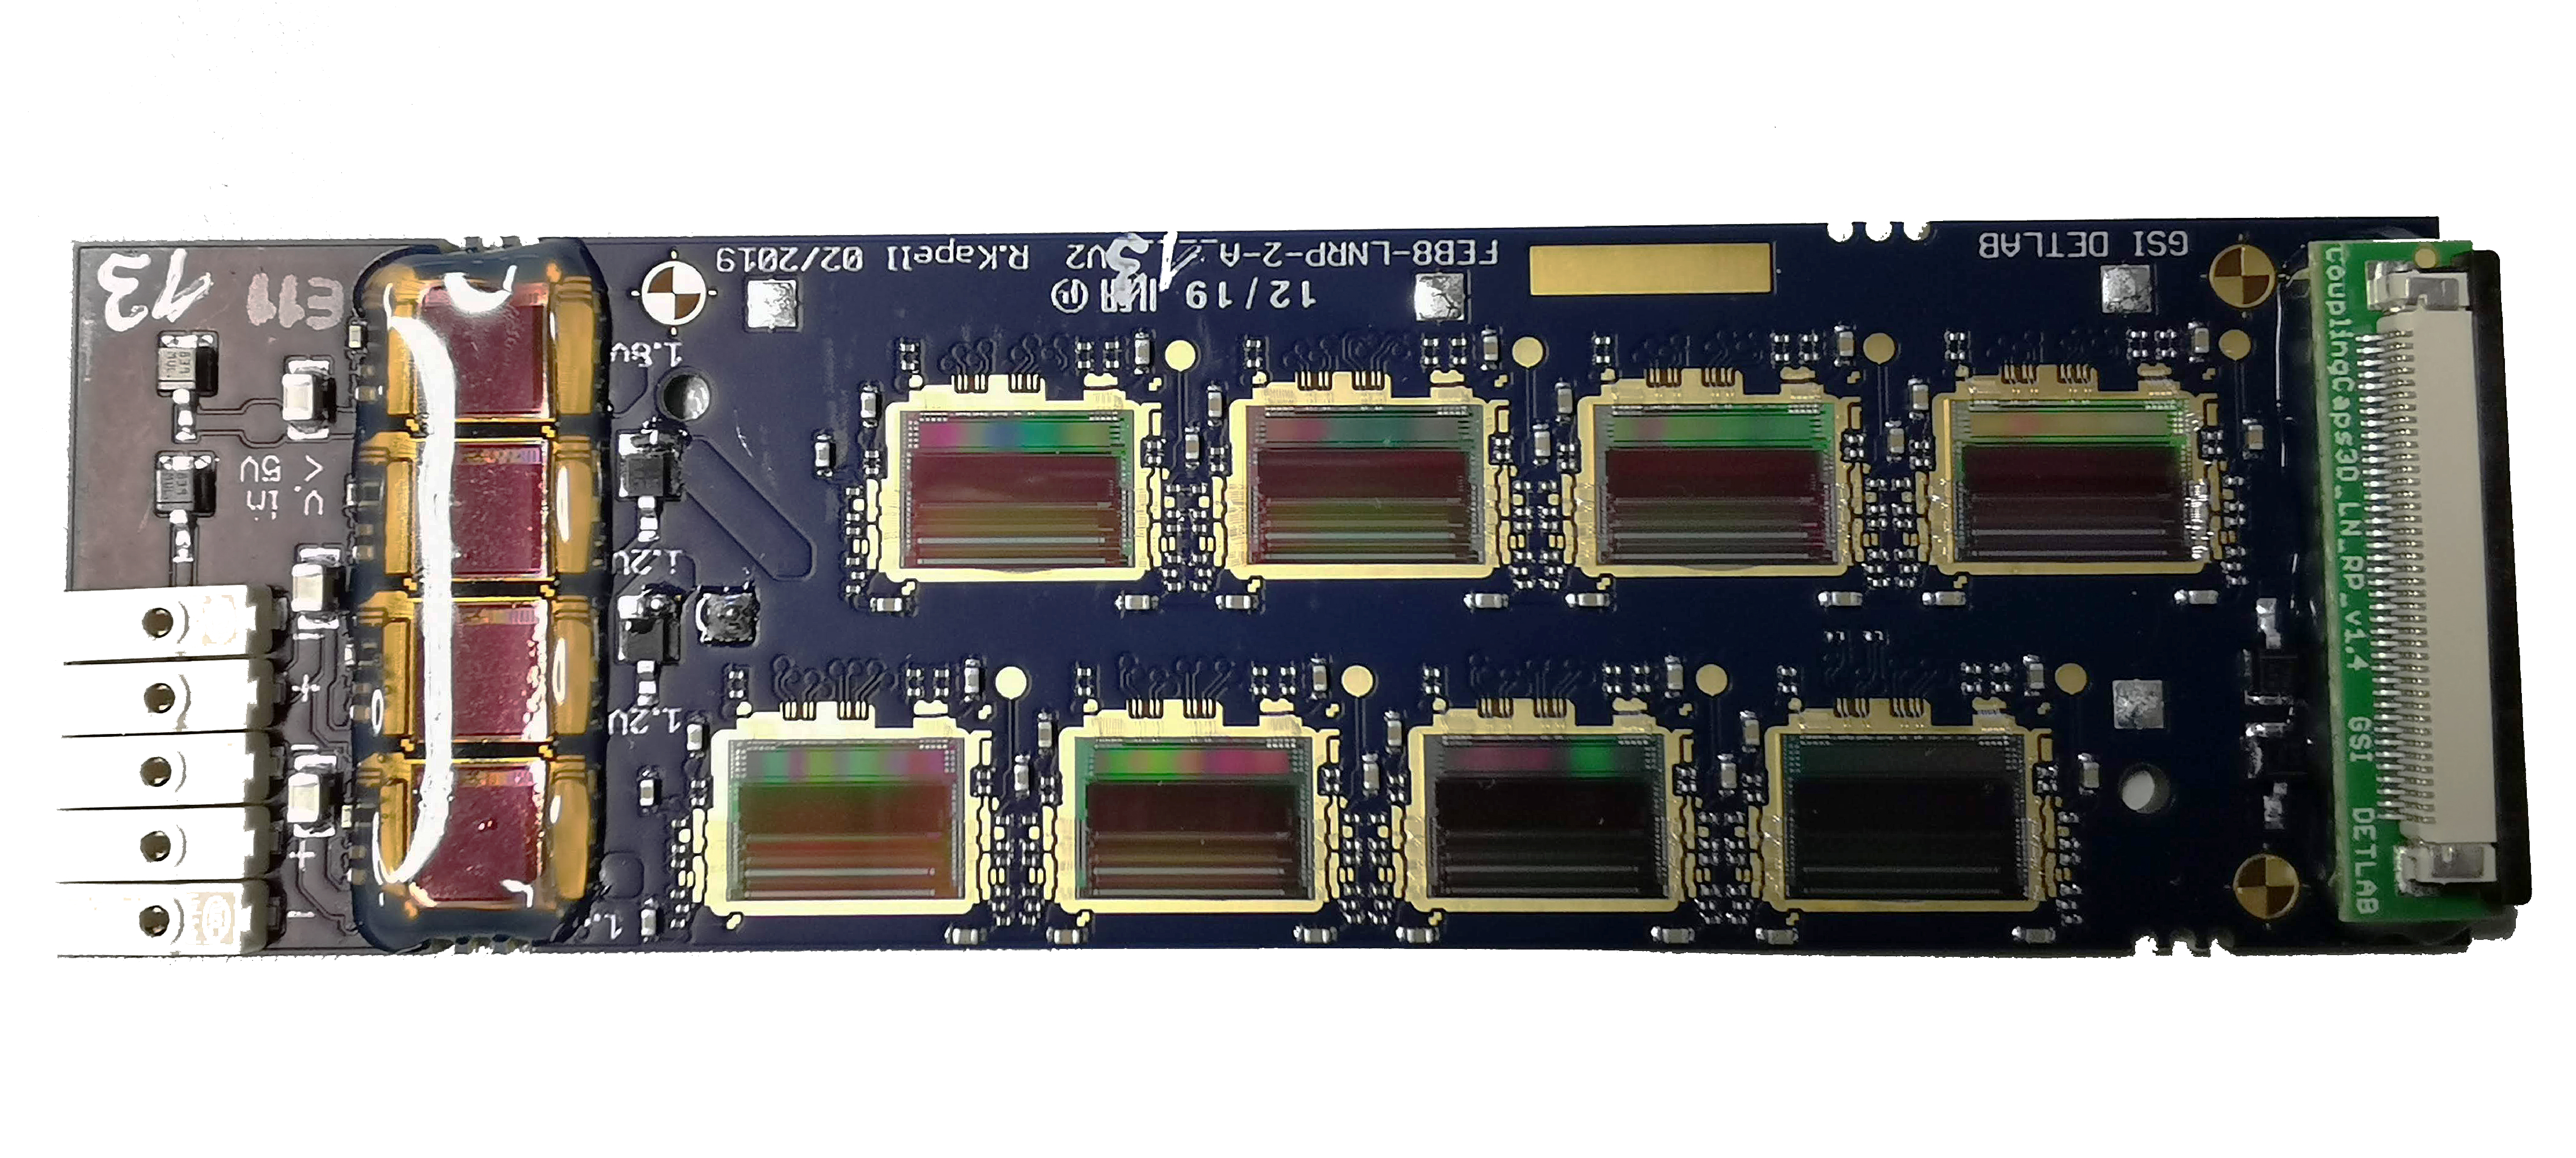
\includegraphics[width=0.65\columnwidth]{Chapter2/images/feb_8_v2.pdf}
\caption{FEB}
\label{fig_febA_photo}
\end{figure}
\subsection{CRI based readout chain}
\begin{figure}[!h]
\centering
\includegraphics[width=0.65\columnwidth]{Chapter2/images/cri_board_atlas.pdf}
\caption{CRI board}
\label{fig_cri_board}
\end{figure}

\label{tester}
Another alternative to the two readout chains introduced in the last two sections is the so-called GBTxEMU-based tester. It is based on a commercial Artix-7 board (TE-0712, Trenz Electronics Gmbh), and allows emulating GBTX ASIC or the whole CROB. Moreover, it could also be used in an autonomous mode with the addition of VITA  57.1 FMC adapter
\subsection{Powering schematics of the detector}
\label{powering}
\subsection{Cooling concept for the STS's electronics and silicon sensors}
\label{cooling}

\subsection{Detector enclosure and its importance}
\section{System safety and the consequences}
\subsection{Requirements for the control system}
\label{sys:req}
Custom solutions that are applied in \gls{STS} make the control of this system very challenging. Different services imply different control solutions which need to be implemented.
A distributed control system should offer remote control, alarm detection, reporting and logging, modeling and simulation, data processing (archiving, retrieval, plotting, conversion, analysis), common time management, access security, and automatic \footnote{Sequencing, also known as sequential control, it controls the device in a pre-determined order.}{sequencing}.
In addition to that, the \gls{DCS} for the Silicon Tracking System (\gls{STS}) is being designed taking into consideration the following aspects:

 
 \begin{itemize}
    \item potential control framework should offer the possibility to control a variety of different services, which often have different communication protocols,
    \item logging, and monitoring - there should be reliable means of supervision of processes, containers, and \footnote{The input/output controller is a device that interfaces between an input or output device and the computer or hardware device}{Input/Output Controllers} (\glspl{IOC}).
    \item the control software should be horizontally and vertically scalable, when it comes to adding additional computing nodes or applications/Input Output Controllers (\glspl{IOC})/containers,
    \item supervision - it should be possible to integrate a sub-system oriented with higher-level control structures,
     \item flexible - applications should be easy to run on different operating systems and processor architectures,
     \item sustainability and support - the experiment is supposed to run for about 10 years, excluding the building and commissioning time. The control system should be sustainable and long-term support provided,
     \item reliability - the system should be highly available, minimizing the downtimes,
     \item network separation - it should be running in a dedicated network (divided into several service-oriented subnets) to have a good overview of the processes and communication between the nodes,
     \item \glspl{GUI} - all parameters/\footnote{In control theory, a process variable is the currently measured value of a particular part of a process which is being monitored or controlled}{process variables} should be available in a user-friendly Graphical User Interface (\gls{GUI}). In case of error or malfunction, it should be stated clearly by the software where the error happened, what could be the potential risk and what actions need to be taken.

 \end{itemize}
\newpage


\chapter{Online systems in the CBM experiment}

As mentioned in Chapter \ref{chap:CBM_STS}, \gls{CBM} will face an unprecedented interaction rate in heavy-ion experiments (up to $10^{7}$~events/s). That number also sets a clear requirement for the detector systems and their corresponding data acquisition. Certain design decisions had to be made to reduce the amount of raw data coming from the subsystems due to the huge quantity of incoming data.

Experiments like \gls{CMS}, use a trigger to \cite{CMS-DAQ} reduce the amount of raw data coming from millions of proton-proton collisions.  In the case of \gls{CBM}, to reduce the data amount, the raw data needs to be evaluated in software on Central Processing Unit (\gls{CPU}) and/or Graphics Processing Unit (\gls{GPU}) level. The self-triggered readout system implies that the association of data from different detectors to individual physical collision events must be based solely on their timestamp, which is generated in the frond-end electronic (\gls{FEE}) circuitry. As a result, a central timing system must synchronize the \gls{FEE} elements to sub-nanosecond precision. On the other hand, the typical event-building action and the high-level trigger are transitioned to the \gls{FLES} (First-level Event Selector) online computing farm. 


\begin{figure}[!h]
\centering
\includegraphics[width=0.7\columnwidth]{Chapter3/Controls/images/online.png}
\caption{General schematics of the CBM readout systems without detector detector specific systems.}
\label{fig_controls}
\end{figure}

\newpage
The readout hardware is connected to the computing farm via custom-developed optical links that manage clock and time distribution, data transfer, and control communication. The Common Readout Interface (\gls{CRI}) connects the links to the online farm. The \gls{CRI} forwards the clock and time information obtained from the Timing and Fast Control (\gls{TFC}) system to the detector \gls{FEE}, and also converts the data received from the detector. Figure~\ref{fig_controls} shows the schematic view of the controls and data acquisition chain of the \gls{CBM} experiment. The Experiment Control System (\gls{ECS}) highlighted in red is also the supervisory structure of the Detector Control System (\gls{DCS}) which controls and monitors the subsystems. The next sections focus on the software components related to the \gls{ECS}, and a detailed explanation of the experiment control with its design. The main focus of the recent work is put on the \gls{DCS}. An introduction to the modern control system frameworks is given, together with a detailed explanation of the functionalities of the specific software components. 
%\newpage
\section{Controlling the CBM experiment}

Heavy-ion physics experiments require complex control systems, which are crucial to the successful operation of the detector system. Proper implementation of such systems ensures an understanding of the safety margins and enhanced data production quality. In general, the whole system should be robust, partitioned, modular, distributed, and highly available. Similar topics were also considered while designing the \gls{STS} control system.

Figure \ref{fig_sim} depicts the targeted control architecture of the future \gls{CBM} experiment. It consists of different software agents\footnote{A software agent is a persistent, goal-oriented computer program.} with clearly defined tasks. During the Phase - 0 experiment of the \gls{CBM} (\gls{mCBM}) some parts of the future \gls{ECS} were tested. The respective parts of the controls have been tested in a standalone mode, which means that there has not been any structured communication between \gls{DCS}, Device Control Agent (\gls{DCA}), and Experiment Control System (\gls{ECS}). Nevertheless, for the final experiment, the detector control system should provide the information on the detector state to the agents residing at a higher level in the control hierarchy and also request the state of the~\gls{DAQ}.

%\newpage
\begin{figure}[!h]
\centering
\includegraphics[width=0.8\columnwidth]{Chapter3/Controls/images/AgentsRelations_V2.pdf}
\caption{\gls{ECS} core agent relations. The numbers and letters indicate how many instances of agents or systems can run concurrently.}
\label{fig_sim}
\end{figure}

 In the next sections, the main features of the control agents are discussed, in particular those that can influence \gls{DCS} (Partition Control Agent (\gls{PCA}), System Control Agent (\gls{SCA}), and \gls{DCA}). Apart from the mentioned agents, the following components are expected to be the part of the experiment controls architecture: 
 \begin{itemize}
     \item Logging and monitoring system - state or configuration changes should be documented for possible revision.
     \item First Level Event Selector network (FLESnet) - \gls{DAQ} software controlling the data readout and timeslice building.
     \item Online processing - software receiving the data from the FLESnet and processing it,
     \item Time and Fast Control (\gls{TFC}) - hardware source of timing information.
 \end{itemize}
\section{Experiment Control System and its structure}\label{sssAgents}

The highest supervisory element of the control strategy is the Experiment Control Agent (\gls{ECA}). It is the top layer of the \gls{ECS}, which should be constantly running and keeping track of the  partitions, the systems in partitions, and the systems out of partitions. 


The \gls{PCA}, is the bottom layer of the \gls{ECS}, which tracks the state and controls a set of detector systems plus all needed central systems. Multiple partitions can run concurrently, potentially allowing for parallel runs with independent detector system sets. Partition (controlled by \gls{PCA}) is a component of the \gls{ECS} describing the combined state of a set of detector systems participating in a common readout. It is used to segment the readout and data flow. It also manages the states of central systems, which do not have partition-level states (e.g. \gls{TFC}, \gls{FLES} in case it does not use internal partitions).  It provides the address and port required by agents to establish the 0MQ\footnote{0MQ is an asynchronous messaging library \cite{zeromq}.} sockets\footnote{A socket is used by a client to send requests to and receive replies from a service.} and build the \gls{ECS} structure upon request.

The \glspl{PCA} hold internal instances of the necessary System Control Agent (\gls{SCA}) interfaces, which are responsible for:
\begin{itemize}
 \item Holding a copy of the current state of the \gls{SCA}.
 \item Periodic ping of the \gls{SCA} to ensure early disconnection detection.
 \item Sending requests to the \gls{SCA} and receiving the replies.
 \item Monitoring the \gls{SCA} broadcast channel for unexpected state changes.
\end{itemize}

These should not be confused with the \gls{SCA}, which are in separate processes (the list will be dynamic and generic at \gls{PCA} level, and can depend on the systems participating in the readout activities): \gls{BMON}, \gls{MVD}, \gls{STS}, \gls{RICH}, \gls{MUCH}, \gls{TRD}, \gls{TOF}, \gls{PSD}. 

The SCA is the first detector supervisory layer, which contains the current information about the state of the \gls{DAQ} and \gls{DCS}. Its role in division into the underlying systems is discussed in the next subsection.

\subsection{System Control Agent and its role}
The subsystem-specific \gls{SCA} should manage communication both with the detector-specific agents and with the higher supervisory entities of \gls{ECS}. Furthermore, \gls{SCA} should provide higher control levels with the global state whenever it is requested, handle any changes reported by a detector (tracking the state), and provide an interface for the shift crew to monitor the state of the system. 

Two main links of the \gls{SCA} include:
\begin{itemize}
    \item Detector Control System - Experimental Physics and Industrial Control System \gls{EPICS}~\cite{EPICS} based distributed control system which controls and monitors all the hardware connected to the specific detector (apart from the \gls{DAQ} specific boards).
    \item Device Control Agent (\gls{DCA}) - this agent controls almost all logic on the \gls{CRI} board (excluding the FLES Interface Module (\gls{FLIM}) section and direct memory access data path). \gls{DCA} provides a high-level interface for the higher layers of the control architecture, collectively referred to as \gls{EDC}. 
\end{itemize}











\section{Controlling a detector}

Data acquisition, parameter monitoring, control, logging, and storage are compulsory tasks for every experimental setup, especially in remote locations with elevated radiation levels. To ensure the safe operation of a detector subsystem automation processes are commonly implemented (e.g. in form of a Finite State Machine \gls{FSM} or hardware interlocks). In the case of \gls{STS}, to ease the use and implementation of a control system, a fairly novel approach was used. It is primarily based on the \footnote{Containerization is the packaging of software code with just the operating system libraries and dependencies required to run the code.}{containerization} of different applications used to monitor and control setups. 

%\begin{figure}[!h]
%\centering
%\includegraphics[width=0.55\columnwidth]{Chapter3/Controls/images/example.png}
%\caption{General detector control system architecture}
%\label{fig_DCS_arch}
%\end{figure}
The control system must provide not only means of communicating between the hardware and software layers but also visualization, logging, archiving, and controlling means (either in an automated way by a Finite State Machine (\gls{FSM}) or manually). The control system can be usually divided into three layers: field layer, control layer, and supervisory layer. The bottom (field) layer contains all the process sensors, actuators, and other devices that are connected to the control system via I/O boards and/or field buses. Communication between the field layer and control layer can be of almost any type compatible with the used components, i.e. Ethernet, Modbus TCP, Profibus. The control logic is introduced in \glspl{PLC} and so-called control nodes (single board computers etc.) in the control layer. The supervision layer or supervisory level provides the operators with means of controlling and monitoring the subsystem, for example via command line or a Graphical User Interface (\gls{GUI}) or Operator Interface (\gls{OPI}) \cite{layers}.  Typically, DCS's building blocks reside in a dedicated network to avoid unnecessary cross-talk and ensure more efficient debugging.

Figure \ref{fig_arch} shows a general idea behind the \gls{STS}'s \gls{DCS} from the software point of view.  The master node or the central \gls{DCS} node gets the data from the configuration database, which will allow the preparation of subsystems for a given action (for example for a transition into a different state). The master node will be only accessible by the \gls{DCS} experts, excluding subsystem-related personnel from performing actions on other subsystems' \gls{DCS}. There are also one or more archiving nodes and control nodes, which will contain detector-specific applications. All the mentioned components allow effective control over a detector and deliver crucial operational information (alarms, events, \glspl{PV} values, etc.). 

\begin{figure}[!h]
\centering
\includegraphics[width=1\columnwidth]{Chapter3/Controls/images/DCS.png}
\caption{Proposed \gls{DCS} infrastructure for the \gls{STS}}
\label{fig_arch}
\end{figure}
\newpage








%empty page
%\newpage
%\thispagestyle{empty} 
%\mbox{}

%\clearpage
%\pagenumbering{arabic}


%%% Insert here the text body, replacing the dummy content.
%\label{sec:introduction
\subsection{Control system for the CBM experiment}
\gls{EPICS} was chosen, as a software platform to implement the \gls{CBM} \gls{DCS}. More detailed explanations of how \gls{EPICS} works are described in the next sections. According to \cite{EPICS_DOCS}, the basic attributes of \gls{EPICS} are:
\begin{itemize}
    \item tool based -- minimized need for custom coding,
    \item distributed -- an arbitrary number of \glspl{IOC} and \glspl{OPI}, as long as the network does not saturate,
    \item event driven -- it is designed to be event-driven to the maximum extent possible,
    \item high performance, robust,
    \item scalable,
    \item under constant development (see latest updates related to the Control System Studio and PVA).
\end{itemize}




%\section{How to control a detector?}

\subsection{What is EPICS?} 
\label{EPICS}
EPICS is a set of tools and applications which provide a software infrastructure for distributed control systems \cite{EPICS_license}. This framework could be used for large systems like particle accelerators, telescopes, etc. as well as for smaller systems featuring only several hundred process variables \cite{EPICS_1, EPICS_2, EPICS_3, EPICS_4}.
\begin{figure}[!h]
\centering
\includegraphics[width=0.7\columnwidth]{Chapter3/Controls/images/EPICS.png}
\caption{EPICS working principle}
\label{fig_EPICS}
\end{figure}
As described in Figure \ref{fig_EPICS}, the system uses client/server and publish/subscribe approaches to communicate between different devices/nodes. Most servers, called Input/Output Controllers ( \gls{IOC}) perform I/O and local control tasks and publish this information to clients via dedicated protocols Channel Access and/or pvAccess \cite{EPICS}. 

 \subsection{Available control tool sets}
 EPICS and related toolkits offer a complete set of applications to control large experiments. Many different sites all over the world have implemented EPICS-based control systems, i.e. \gls{J-PARC} \cite{J-PARC}, \gls{STAR} \cite{STAR}, \gls{ITER} \cite{ITER}, Australian Synchrotron and many more \cite{EPICS_site}. Besides, there are also different alternatives to implementing a control system, which include: 
 \begin{itemize}
     \item Siemens WinCC \cite{Camacho:2022fxa,Goralczyk:2022udx}
     \item Tango \cite{Santander-Vela:2021tma}
     \item Labview \cite{State:2022qlw} 
     \item custom software (e.g. python/C++ or stream processing software) \cite{taurus}
 \end{itemize} 
 These frameworks were discarded either because of licensing needs (Labview, Siemens WinCC) or lack of extensive experience on-site (Tango). Phoebus \cite{Phoebus} was chosen as the collection of tools and applications to monitor and operate \gls{STS}. All \gls{mSTS}'s \glspl{OPI} were prepared in Phoebus \cite{Phoebus}. The detector uses the following Phoebus-related applications:
\begin{itemize}
    \item Alarms logging
    \item Alarm server
    \item Save and restore
\end{itemize}
More details about these applications and their use will be provided in the next sections. Although Phoebus proved to be easy to use and implement new operator screens, there are also alternatives that could provide similar functionalities:
\begin{itemize}
    \item Bluesky Project (Python-based set of libraries \cite{Bluesky}),
    \item React Automation Studio \cite{React},
    \item Channel Access Tools - MEDM, \gls{ALH}, \gls{AR} etc. 
\end{itemize}

\subsection{EPICS architecture and IOC}
The core elements of the systems are the \glspl{IOC}, which provides control logic for the connected hardware. The \gls{IOC} uses channel access and/or PVAccess to communicate with clients and contains also the following parts\cite{IOC}:
\begin{itemize}
    \item \gls{IOC} database -  a memory resident database containing a set of named records of various types \cite{IOC2},
    \item record support - set of support routines defining a record,
    \item device support and drivers - serve access to external devices.
    \item monitors and scanners,
    \item sequencer - an optional extension of the \gls{IOC} which is a finite state machine,
\end{itemize}
An \gls{IOC} doesn't need extensive computing resources, that's why it runs also on low-power single-board computers like Raspberry PI or Odroid. 
 \gls{IOC} are also commonly supported by additional modules, device support, libraries, and \glspl{API} which altogether provide an efficient way to control various devices.
To communicate with devices, an \gls{IOC} uses so-called device support. The most commonly used ones include:
\begin{itemize}
    \item StreamDevice is a generic EPICS device support for devices with a "byte stream" based communication interface. That means devices that can be controlled by sending and receiving strings (in the broadest sense, including non-printable characters and even null-bytes). Examples of this type of communication interface are serial line (RS-232, RS-485, ...), IEEE-488 (also known as GPIB or HP-IB), and telnet-like TCP/IP \cite{StreamDevice},
    \item devModbus \cite{modbus} - includes support for three Modbus standards (TCP, RTU, ASCII), used for control of climatic chambers in the \gls{STS} group,
    \item asynDriver \cite{asyn} - asynchronous driver support, which is an interface that implements a device-specific code to low-level communication drivers. Together with the StreamDevice it's the most commonly used one in the \gls{mSTS}. 
\end{itemize}

In order to ease the deployment process and have a flexible solution for different architectures, images for the \gls{IOC} as well as other \gls{DCS} building blocks were created. These images can be seen as files with code that upon execution result in the initialization of a container. More detailed information about containerization is included in the next chapter. 
 


%\chapter{Containerized control software and its applications}
\chapter{Containerized control software and its applications}
\label{containers}
The \gls{EPICS} and related toolkits can be used to control large experiments or even beamlines, but also smaller experimental setups, in which only a limited functionalities are needed. During the R\&D phase for the \gls{STS} many different setups were constructed, in order to evaluate the hardware that should be used for the final experiment. Moreover, challenging ambient conditions of the STS put even more stringent constraints. To address the needs of this dynamic environment, a container based control framework was implemented. 

Containerization is an increasingly popular method of virtualizing an application, without having to run a full-blown operating system. In modern computing, containers are commonly used both in development and production environments, often together with cloud solutions. In the \gls{HEP} containers and their different applications become more and more popular. According to~\cite{Klaus2021} the first mention of about a docker container of the \gls{EPICS} \gls{IOC} was related to the Taurus project in 2015~\cite{taurus}. Since then containerization efforts intensified also within the \gls{FAIR} based collaborations - \gls{CBM}/\gls{MVD}~\cite{Klaus2021} and PANDA DCS~\cite{PANDA_1}.

In this chapter, an introduction to the modern control system frameworks is given, together with a detailed explanation of the functionalities of the specific software components. Two following sections introduce the applications of the developed software package for the effective control and data acquisition in two chosen setups. The first of mentioned sections focuses on the powering irradiation studies and implications for the STS. The last section discusses the results from the thermal cycling activities for the STS electronics, that aimed to discover their operational limitations.
  
\section{Containerized IOC}
IOC container has been prepared by the \gls{DCS} group of the \gls{PANDA} Collaboration and adjusted to the STS needs. The latest IOC's image is built on EPICS R7.0.3.1 image and it contains the most important modules and extensions i.a. asyn, autosave, calc, modbus and SNMP (see Figure~\ref{fig_ioc1}). Moreover, by using so-called Volumes (see Figure~\ref{fig_doc}) the \gls{IOC} can be used at any node with docker engine. Volumes are one of the mechanisms to manage application data and it's a proper way to ensure data persistence. Having prepared database files, st.cmd, and stream protocols if needed, an IOC can be deployed on any node, with any operating system and processor architecture.
\begin{figure}[!h]
\centering
\includegraphics[width=0.65\columnwidth]{Chapter3/DCS/images/epics_ioc.png}
\caption{EPICS 7.0.3.1 based IOC image}
\label{fig_ioc1}
\end{figure}
\newpage
A general idea of an containerized \gls{EPICS} \gls{IOC} is presented in the Figure~\ref{fig_doc}. Every container is assigned an IP address for every Docker network it connects to. Moreover, each network has a default subnet mask and gateway. In order to connect the IOC with other services, the ports used by \gls{EPICS} (5064, 5065 for channel access protocol and 7064, 7065 for PVAccess) need to be exposed.  The containers use the host network to communicate with each other and other nodes. It's mostly due to limitations in the protocols used by the \gls{IOC}, as they may not pass through Network Address Translation (NAT).
\begin{figure}[!h]
\centering
\includegraphics[width=0.7\columnwidth]{Chapter3/DCS/images/docker_run.png}
\caption{General idea of an IOC in the container}
\label{fig_doc}
\end{figure}
\newpage
\section{Docker}
Docker was chosen as the platform to prepare the images and run the containers. One of the features of docker has been considered risky for the operation of the detector/experiment, especially considering the final system. Docker-based containers run with the root privileges, therefore posing a threat to the operation of the control system. The daemon is a part of the engine that runs the containers that have full privileges not only within the container but also on the node. If a container gets compromised it may lead to potentially disastrous scenarios, including loss of data or potential threat to the detector - e.g. killing the container. Moreover, a compromised node can also endanger other nodes in the network.  Nevertheless, since late 2020 it's possible to run Docker daemon and containers as a non-root user. Docker daemon and containers themselves can run inside a user namespace~\cite{docker_limitations}, therefore mitigating risk
%\begin{figure}[!h]
%\centering
%\includegraphics[width=0.8\columnwidth]{sections/images/docker.png}
%\caption{Rootless operation of the container}
%\label{fig_rootless}
%\end{figure}
 Thanks to the Open Container Initiative that defines container formats and runtimes, using different engines doesn't require many changes in the container image. There are also several alternatives to the docker engine, that allow running containers in rootless mode:
\begin{itemize}
    \item Podman~\cite{Podman} 
    \item Singularity~\cite{singularity}
\end{itemize}
\section{Safety Considerations}
Containers are a handy tool to easily address the control and monitoring of different setups. Nevertheless, implementing an additional layer over EPICS-based applications may lead to safety concerns. This technology has many advantages:
\begin{itemize}
    \item standardized, what makes it portable anywhere,
    \item independent of the operating system,
    \item instant replication and easy debugging,
    \item lightweight - containers share the machine's kernel, and they do not require a separate one, which makes them much faster than virtual machines,
    \item docker daemon monitors the containers instead of the hypervisor in case of virtual machines,
    \item processes run as native causing little overhead.
\end{itemize}
For the use of containers in the final experiment, the following list must be taken into consideration:

\begin{itemize}
    \item services should be accessible only by experts, crucial services should be hidden from operators (authorization),
    \item ssh accesses to the DCS nodes should be limited by authorization plugins to avoid overloading,
    \item experiment network should be segmented based on the goals and communication between software entities clearly, defined (\gls{DCS}, \gls{SCA})
    \item proper security context for all the services (e.g. root privileges),
    \item logging all the changes in the cluster,
    \item preventing containers from loading unwanted kernel modules,
    \item cluster and container redundancy.
\end{itemize}

\section{Motivation}
Nevertheless, to demonstrate the containerized \gls{DCS}, not all the available applications were used. The mSTS's \gls{DCS} features the applications listed in the figure \ref{fig_dcs_node_msts}. All these applications were used as containers based on previously prepared images and linked using Docker-compose, which is a tool for defining and running multi-container Docker applications \cite{docker_compose}. To configure the containers a YAML file has to be populated with the container settings. This section summarizes the most important applications used for the DCS and their functionalities.

\section{Multi-container applications}
Over the years \gls{EPICS} has become a framework that offers users many off-the-shelf applications that ease the implementation and configuration of a control system. Figure \ref{fig_dcs_node_msts} shows the most commonly used control-related applications. 

All the applications in figure~\ref{fig_dcs_node_msts} applications were used as containers based on prepared images and linked using Docker-compose, which is a tool for defining and running multi-container Docker applications~\cite{docker_compose}. To configure the containers a \footnote{YAML is a human-friendly data serialization language for all programming languages~\cite{YAML}.}{YAML} file has to be populated with the services settings (in this case the services refer to the applications, e.g. \gls{IOC}. This section summarizes the most important applications used for the \gls{DCS} and their functionalities.


\begin{figure}[!h]
\centering
\includegraphics[width=0.95\columnwidth]{Chapter4/images/dcs_node.jpg}
\caption{Services used in addition to Phoebus functionalities, together forming a full-blown control system.}
\label{fig_dcs_node_msts}
\end{figure}
\newpage
\subsection{Control System Studio and Phoebus}

Control System Studio (\gls{CSS}) consists of open-source Java applications and modules which can be used in constructing a control system. Phoebus is an update to the \gls{CSS} and significantly improves its performance by removing dependencies on Eclipse RCP. Phoebus uses both channel access protocol and \gls{PV} access and it offers graphically based applications to access \gls{EPICS} \glspl{PV}, \glspl{OPI}, PVs history, etc. An example of a chiller \gls{GUI} is depicted in figure~\ref{fig_lauda1}. One of the main features of Phoebus is its modular nature. Users can develop and add their products or just include or exclude applications or configurations. 


\begin{figure}[!h]
\centering
\includegraphics[width=0.92\columnwidth]{Chapter4/images/lauda1.png}
\caption{An example of a detector system \gls{GUI}.}
\label{fig_lauda1}
\end{figure}

\newpage
\subsection{Archiver Solutions} \label{archiver}
An Archiver serves as one of the main building blocks of the \gls{DCS}, as it allows not only to look up the history of a given record but also to download and post-process the data. Archivers make use of the publish/subscribe logic, updating the values on change. In general, the archiver must run smoothly, without significant downtime, and the linked database and other clients should also have a stable connection. A primary choice for \gls{STS} is the so-called Archiver Appliance~\cite{archiver_appliance}. An example of the archiver appliance is divided into short-term storage, medium-term storage, and long-term storage. In principle a system administrator can adjust these settings to the needs of the specific case. The  four \footnote{An Open source web server by the Apache foundation}{Tomcat containers } are employed to handle the tasks of the archiver.  
%\begin{figure}[!h]
%\centering
%\includegraphics[width=0.7\columnwidth]{Chapter4/images/applarch.png}
%\caption{Architecture of a single appliance \cite{archiver_appliance}}
%\label{fig_archiver}
%\end{figure}
%\newline

The main advantage of the archiver include: 

\begin{itemize}
    \item Data retrieval can be integrated into Phoebus or Matlab,
    \item Wide range of supported formats,
    \item stable performance, even with a hundred thousand \glspl{PV}.
\end{itemize}

Apart from the Archiver appliance, there are also alternative solutions:

\begin{itemize}
    \item Cassandra \cite{cassandra_archive},
    \item RDB Archive engine \cite{rdb_archive}.
\end{itemize}

\subsection{Alarm server}
An alarm server monitors a chosen set of \glspl{PV}, including their alarm state. \gls{EPICS} records facilitate fields related to the alarm thresholds and their severity, evaluated each time the record is processed. Every numeric value could have two uppers and two lower boundaries, with assigned severities (NO\_ALARM, MINOR, MAJOR). \gls{EPICS} by itself doesn't take any actions on the detector's hardware when the alarm threshold is exceeded. On the other hand, a Phoebus-based \gls{GUI} will change the font color (MINOR - orange, MAJOR - red) of the variable once the alarm appears. If the connection to the alarm server exists, then the server acts upon a change in the alarm status of a record. The user interfaces show alarms, allow acknowledgment, and provide guidance and helpful links. Apache Kafka is a distributed event store and stream-processing platform which serves as a communication bus between the alarm server and Phoebus. An example of the \gls{mSTS}'s alarm handling \gls{GUI} is depicted in Figure~\ref{fig_alarm1}. It provides not only a visual notification of an alarm but also guidance, displays, and commands.
\begin{figure}[!h]
\centering
\includegraphics[width=1\columnwidth]{Chapter4/images/alarms.png}
\caption{Phoebus alarm handler view -  top left part some \gls{GUI}s, the top right part is the alarm table showing the current and acknowledged alarms, bottom left features a color status of respective nodes (e.g. cooling), bottom right shows the latest entries in the log}
\label{fig_alarm1}
\end{figure}
\newpage
\subsection{Alarm logging}
Logging is another important part of the \gls{DCS}. It allows monitoring and checking of all the changes in the configuration and alarms of all the process variables. Thanks to the logs acquired by the dedicated service, debugging becomes much easier. The alarm logging service enables the logging of: configuration changes, state changes logging, and commands. Similarly to the alarm server, it uses Apache Kafka for data transfer. Apart from the logs, there is also a \gls{GUI} available in the Phoebus \cite{alarm_logger}, an operator can also use the \footnote{source-available data visualization dashboard software }{Kibana} web interface to discover patterns and trends in the data. 

\subsection{Finite state machine}
A finite state machine (\gls{FSM}) is a construct that defines states and transitions between these states. In a given moment it has a clearly defined state and a given set of rules and conditions apply to this state. An input issued by an operator or automatically by a sensor(s) could trigger a transition. All transitions are unidirectional, but it's possible to define two opposite transitions, e.g. entering and escaping the error state. 
\newpage
One of the possibilities to implement a \gls{FSM} is to use Sequencer, which is a State Notation Language based on C/C++. 
\begin{itemize}
    \item start-up, shut-down, fault recovery, etc.,
    \item little C code, many states, many transitions,
    \item short compilation time, and can call any C++ code, easy connection to channelAccess.
\end{itemize}

One of the alternatives to the Sequencer and State Notation language is the PyEPICS-based library Pysmlib. It features several interesting functions like integrated watchdog logic, multi-threading, or configurable logging systems.


\section{Containerized EPICS-based framework}

The containers based framework introduced in this chapter is the baseline for all the research and development activities throughout this thesis. In principle, most small and/or laboratory based experimental setups don't require a full-blown control systems. Hence, in the next two chapters two smaller framework applications will be introduced. In addition to that, the studies and their implications are discussed in detail. Chapter 6 is dedicated to the application of the full control system to the Phase-0 version of the \gls{STS}.
\section{Monitoring of the Frond End Electronics}
The first application of the introduced control framework was to read out several parameters from different readout chains (see section \ref{readout} for a detailed explanation of different readout chains). The \gls{ROB} and \gls{DPB} based readout chain was mostly used to evaluate the possibility of interfacing the values from the \gls{DAQ} chain to the slow control and \gls{EPICS} based system. The purpose, similarly to the GBTxEMU chain, was to monitor the stability of the readouts throughout different tests, e.g. thermal cycling of the \gls{FEE}. A maximum of 2 FEBs - 16 STS-XYTERs were used, so in total 112 process variables were monitored, which makes it a small setup. Those values were then stored in a database and are available from Phoebus. 

The available parameters included those available from \gls{GBT} \gls{SCA2} \gls{ASIC} \cite{GBT_SCA_ASIC} and three GBTX chips: 
\begin{itemize}
    \item GBT SCA - RSSI (Received Single Strength Indicator), Input voltage $V_{in}$, 1.5V DC/DC converter output voltage $V_{out}$, 2.5V DC/DC converter output voltage $V_{out}$ (see figure \ref{fig:ROB}), two temperature sensors
    \item GBTX \gls{ASIC} - FEC (Forward Error Correction) counts
\end{itemize}
%\newpage

\begin{figure}[!h]
    \centering
    \includegraphics[width=0.65\columnwidth]{Chapter3/FEE/images/ROB.png}
    \caption{$V_{out}$ output voltage from one of the DC/DC converters in the \gls{ROB}}
    \label{fig:ROB}
\end{figure}

The STS-XYTER provides the following values - almost full counter, event missed counter, single event upset counter, the status register, and \gls{DAC} values: $V_{ddm}$, \gls{CSA} bias, temperature. 

\begin{figure}[!h]
    \centering
    \includegraphics[width=0.65\columnwidth]{Chapter3/FEE/images/FEB.png}
    \caption{$V_{ddm}$ readouts from the diagnostic circuits of two ASICs}
    \label{fig:vddm_first}
\end{figure}

FEE monitoring plays a crucial role in the detector operation but also during the testing phase. Internal parameters of the ASICs in the \gls{ROB} or \gls{FEB} deliver information about the stability and onset of failure. %\subsection{Parameters of the STS-XYTERv2 ASIC}
%\subsection{GBTX and GBT ASIC monitoring}
%\newpage
\section{Irradiation studies of the powering units}
Radiation-induced effects in electronics play an important role in accelerator facilities, where different particle species may elevate radiation levels even in relatively remote areas. Depending on many factors, i.a. location of the setup, intensity or energy of the incident particles, damage caused to a semiconductor device may vary greatly. A particle could cause no observable effect, transient disruption of circuit operation, a change of logic state, or even permanent damage to the device or integrated circuit (IC)~\cite{dodd}. The detector will be powered by about 140 low voltage modules, providing 2100 power channels. In order to estimate the Single Event Effects (SEE) in the powering electronics in the envisaged radiation environment, two irradiation campaigns took place in GSI, Darmstadt.  The first one was conducted at the mini-CBM experiment and the second was realized next to the electrostatic septum of the SIS18 synchrotron. These irradiation campaigns aimed at detecting radiation-induced soft errors in the power units' electronics and estimating its rate.


\subsection{Single Event Effects in the electronics}
A variety of different elements and chemical compounds can be used in electronics, including silicon, silicon dioxide ($\mathrm{SiO}_{2}$), or boron. The high ambient flux of particles in a particle accelerator environment usually consists of charged particles (mostly protons, and electrons), high-energy photons (gamma and X-rays), and a broad spectrum of neutrons. Different interaction mechanisms may cause both stochastic and deterministic effects in electronics. These effects are directly related to the integrated dose and linear energy transfer (\gls{LET}) of the incident particles ~\cite{electronic_system_on_module}. Radiation-induced soft errors have become a huge concern in advanced computer chips because uncorrected, they produce a failure rate that is higher than all the other mechanisms compromising reliability combined~\cite{1545891}. Neutrons do not cause direct ionization in silicon or oxygen. These neutral particles interact elastically as well as inelastically, resulting either in the creation of other nuclei and the emission of a light particle or in changes in the kinetic energies of the participants. A few neutron threshold energies for reactions with oxygen and silicon are summarized in Table~\ref{cross-seciton}. The cross-section for neutron reactions generally decreases with the energy. Moreover, neutrons can indirectly cause SEE by secondary radiation, for example, a reaction with boron which results in the emission of an $\alpha$ particle $^{10}\mathrm{B}(n,\alpha)^{7}\mathrm{Li}$~\cite{1545891,neutrons_energy,neutrons_energy_2}. 

\begin{table}[!h]
\centering
\begin{tabular}{lc}
\hline
Reaction         & Neutron Threshold Energy (MeV) \\ \hline
Si elastic       & 0                              \\
Si(n,$\alpha$)   & 2.75                           \\
Si(n,p)          & 4                              \\
Si(n,d)          & 10.5                           \\
Si(n,$n-\alpha$) & 10.35                          \\ \hline
O elastic        & 0                              \\
O(n,$\alpha$)    & 2.35                           \\
O(n,$n-\alpha$)  & 7.61                           \\
O(n,p)           & 10.24                          \\
O(n,d)           & 10.53                         
\end{tabular}
\caption{Threshold energies of neutron reactions with silicon and oxygen nuclei~\cite{ENDF}}
\label{cross-seciton}
\end{table}

%\newpage
\subsection{Motivation}

The powering of the Front End Boards (\gls{FEB}s), together with the data processing electronics, sum up to about 2100 low voltage channels, operated in about 140 low voltage modules, 16 channels each. All of them will be placed in a protected area within the cave with an elevated radiation level. The estimated dose values were calculated by A. Senger using FLUKA code (see Figure~\ref{fig:mCBM})~\cite{FLUKA}. 

\begin{figure}[!h]
    \centering
   % \includegraphics[width=0.95\columnwidth]{images/dose3.png}
    \includegraphics[width=0.55\columnwidth]{Chapter3/Irradiation/images/Dose00.jpg}
    \caption{Expected dose distribution in the air in the \gls{CBM}
cave under the platform in (11 AGeV Au $10^{9} \mathrm{\ ions/s}$ on 1\% Au
interaction target) 0 to 0.5 m and 1.5 m to 2 m above the ground} 
    \label{fig:mCBM}
\end{figure}

musiFor the gold beam with the highest available intensities ($10^{9}\mathrm{\ ions/s}$) and energies (11 AGeV), we expect a total dose level of 20 mGy after 1 month of operation in the area between 0 and 0.5 m above the ground (at the planned location of the power crates x = -600 cm, z = -600 cm) and 40 mGy between 1.5 m and 2 m above the ground (x = -600 cm, z = -600 cm). A failure in the low voltage powering of the FEE may lead to a rapid decrease of temperature, as the primary coolant temperature may reach down to $-40^{\circ}\mathrm{C}$, consequently making the FEE susceptible to thermal stress. The effects of radiation must be therefore studied to ensure the safe operation of the STS. Estimation of the soft error rate (\gls{SER}) may also indicate whether there is a need for further shielding of the power electronics in order to minimize the overall dose.


\subsection{Methodology}
The subject of the irradiation campaign was a MPOD mini crate with one low voltage (WIENER) and one high voltage (ISEG) module. The crate's CC24 controller (ISEG) offers an embedded EPICS Input Output controller, which was used to detect radiation-induced channel or module failures. All registered events were stored in a dedicated database. In order to correlate the soft failure rate with the absorbed dose, two types of thermoluminescent dosimeters were used. A larger polyethylene sphere (d = 30 cm) was used to measure the neutron ambient dose, whilst the cylinder (d = 5 cm, h = 6 cm) measured other particles~\cite{bonner}. We assume that the conditions (neutron spectra - mostly thermal neutrons, neutron moderators, etc.) at the \gls{CBM} experiment will be similar to conditions at SIS18, and at the mCBM experiment. Therefore, the quality factor, which takes into account both \gls{LET} and relative biological effectiveness (\gls{RBE}), to convert the measured given in Sv to absorbed energy in Gy is 5 for both irradiation campaigns. The dose measured with the cylinder is assumed to have a quality factor of 1.

\subsection{Poisson distribution}
We assume that failure events (radiation-induced errors) are statistically independent and are driven by purely stochastic factors. Moreover, we take into account only the total dose measured by the dosimeters, thus rapid dose changes and their effect are not investigated in this contribution. In such a case, the probability of observing $n_{m}$ events with the mean value $\mu$ is described by the Poisson distribution:\newline
\begin{equation}
    p(n|\mu) = \frac{\mu^{n}}{n!}e^{-\mu}
\end{equation}
The total number of events is considered to be the average $\mu$, as this is the most reasonable assumption.
Assuming 68\% confidence levels for values $n_{m} > 2$ we can apply the following equations to estimate the distribution's bands (see Figure~\ref{fig:poisson})~\cite{schmidt}.
If in an experiment $\mu$ events are measured, we conclude that the standard deviation is described by $\mu - \sqrt{\mu}$ and $\mu + 1 + \mu$ around the average value $\mu$.
\begin{figure}[!h]
    \centering
    \includegraphics[width=0.55\columnwidth]{Chapter3/Irradiation/images/poisson.png}
    \caption{Estimated bands of the Poisson distribution~\cite{schmidt}}
    \label{fig:poisson}
\end{figure}
%\newpage
For $n_{m} \leq 2$ previously mentioned, estimations do not provide accurate results, therefore upper and lower bands need to be calculated explicitly. According to~\cite{schmidt}:



\begin{table}[!h]
\centering
\begin{tabular}{ccc}
\hline
Number of counts & \multicolumn{2}{c}{Poisonn's distrubution} \\ \cline{2-3} 
$n_{m}$          & $\mu_{l}$            & $\mu_{u}$           \\ \hline
0                & 0                    & 1.84                \\
1                & 0.173                & 3.30                \\
2                & 0.708                & 4.64                \\ \hline
\end{tabular}

\end{table}
\newpage
\subsection{Irradiation at the mCBM experiment}
In order to investigate electronics' operation under the realistic conditions, that low voltage modules will face during the CBM experiment, an irradiation campaign took place at the mCBM experiment (see figure~\ref{fig:CBM1}). Different intensities and reaction systems (Au+Au, Au+Ni, etc.) were exercised during the experiment.
\begin{figure}[!h]
    \centering
    \includegraphics[width=0.55\columnwidth]{Chapter3/Irradiation/images/dose1.jpg}
    \caption{Expected dose rate distribution (mGy/hour) in the mCBM cave with 2 AGeV O ions beam of   $10^{7}\mathrm{\ ions/s}$ on 4 mm Ni target}
     \label{fig:CBM1}
\end{figure}
\begin{figure}[!h]
    \centering
    \includegraphics[width=0.4\columnwidth]{Chapter3/Irradiation/images/crate.jpg}
    \caption{Crate irradiation setup at the mCBM experiment. The photo depicts two TLD dosimeters in the background, and two TLD dosimeters and the crate in the foreground}
    \label{fig:crate}
\end{figure}
\newpage
To measure the dose that the crate was exposed to, four thermoluminescent dosimeters (\gls{TLD}) with moderators were used (Figure~\ref{fig:crate}). Two TLDs placed far away from the crate served as a reference. During the irradiation at the mCBM experiment, the dosimeters were read out twice, in order to evaluate the total dose received by the crate. The first value was $19.72\mathrm{\ mGy}$ and  the second one was $72.31\mathrm{\ mGy}$. 

A \gls{SEE} in the low voltage module occurred in each part of the irradiation. In both cases, it was possible to recover the functionalities by enabling the channels again. In total, $n=2$ after ($92\pm{4.6}\mathrm{\ mGy}$), considering standard 5\% uncertainty for the TLD. After applying lower and upper limits we find:
%\newpage
In total, $n=2$ after ($92\pm{4.6}\mathrm{\ mGy}$).
After applying lower and upper limits we get:
\begin{equation}
    D_{lower}=\frac{92}{0.708} = 129.9\mathrm{\ mGy}
\end{equation}
\begin{equation}
    D_{upper}=\frac{92}{4.64} = 19.8\mathrm{\ mGy}
\end{equation}
The uncertainty for $n_{m}=2$ is extremely high and equals to $\mathrm{46}_{-26}^{+84}$ mGy, therefore no clear conclusion on the behavior of the crate could be made. To further increase the statistics, a second irradiation campaign took place at the electrostatic septum of the SIS18 synchrotron. 
%\vspace{10cm}
\subsection{Irradiation at the SIS18 septum}
\subsubsection{Setup}
The setup at the SIS18's septum consisted of two \gls{TLD} dosimeters (for neutrons and other particles separately). Moreover, the total doses from TLDs were supplemented with readouts from two active dosimeters placed behind the wall (see Figure~\ref{fig:spec_des}). 
\begin{figure}[!ht]
    \centering
    \includegraphics[width=0.45\columnwidth]{Chapter3/Irradiation/images/septum.jpg}
    \caption{Location of the dosimeters and crate at the SIS18. The so-called Kickerraum contained WENDI-2 and Gamma probe, whereas two TLD dosimeters were placed next to the power crate - depicted with a blue dot between segments 6 and 7.}
    \label{fig:spec_des}
\end{figure}

Wendi-2 is a precise wide-energy neutron dosimeter~\cite{wendi} that was used to determine the neutron dose rate in the so-called Kickerraum. Due to the shielding of the wall, the gamma probe measured mostly background radiation. The MPOD mini crate was placed next to the TLD dosimeters. In order to calculate the active neutron dose next to the crate, a ratio of total doses from both measurement places was used. 
\newpage
\subsubsection{Results}
During the irradiation period, readings from the dosimeters reached $106.1\mathrm{\ mSv}$ and $27.7\mathrm{\ mSv}$ for neutrons and other particles respectively.
%(Figure~\ref{fig:spectrum} depicts neutrons spectrum at the irradiation place).
%\begin{figure}[!ht]
%    \centering
%    \includegraphics[width=0.9\columnwidth]{Chapter3/Irradiation/images/fig5.png}
%    \caption{Neutron spectrum at the measurement location (SIS18 septum). It is based on the measurement of argon ions at 550 MeV/u. The first peak is related to the thermal neutrons and %the second one to the fast neutrons}
%    \label{fig:spectrum}
%\end{figure}
Using assumed quality factors, we convert the ambient dose to the absorbed dose values. Hence, we get in total $49\pm{2}\mathrm{\ mGy}$, taking into account 5\% standard uncertainty of the TLD dosimeters. During the irradiation 11 radiation-induced soft failures were identified in the low voltage module. Therefore, we can estimate an average dose after which a low voltage failure might take place.
\begin{figure}[!h]
    \centering
    \includegraphics[width=0.57\columnwidth]{Chapter3/Irradiation/images/LV_failure_and_neutronsrate.png}
    \caption{Cumulative neutron dose and SEE in the low voltage module}
    \label{fig:lv_neutrons}
\end{figure}
\begin{figure}[!h]
    \centering
    \includegraphics[width=0.57\columnwidth]{Chapter3/Irradiation/images/neutrons_dose_rate.png}
    \caption{Neutron dose rate and failures of the low voltage module}
    \label{fig:lv_neutrons_rate}
\end{figure}
Figure~\ref{fig:lv_neutrons} shows how the number of failures cumulative with the total neutron dose, where the longer periods without failure indicate a break in SIS18 operation. Similarly, Figure~\ref{fig:lv_neutrons_rate} depicts the dose rate and related \gls{SEE}.
For the 11 low voltage module failures, we get the following confidence bands from the Poisson distribution:
   \begin{equation}
  \mathrm{\mu}_{\mathrm{LV}}^{\mathrm{SEE}}=\mathrm{11}_{-3}^{+4}
\end{equation}
Considering the sum of two doses, we get:
\begin{equation}
    \mathrm{D}_{\mathrm{LV}}^{\mathrm{SEE}}=\mathrm{4.45}_{-1.25}^{+1.93}\mathrm{\ mGy}
\end{equation}
Therefore, we can expect a low voltage module failure after $\mathrm{4.45}_{-1.25}^{+1.93}\mathrm{\ mGy}.$ After the occurrence of a soft error in the low voltage module, it was always possible to turn the channels on again.
\newpage
On the other hand, high voltage modules will be placed in an area with lower radiation levels, thus their error sensitivity does not pose a risk to detector operation. In the case of the high voltage module, the \gls{SEE} don't result in a module switch off, but in disabling channels. In two cases all channels were switched off, which is counted as if 15 channels were turned off at the same time. Figure \ref{fig:hv_neutrons} and \ref{fig:hv_neutrons_rate} show the channels' failure rate with the increasing cumulative dose. 
\begin{figure}[!h]
    \centering
    \includegraphics[width=0.57\columnwidth]{Chapter3/Irradiation/images/HV_failure_and_neutronrate.png}
    \caption{Cumulative neutron dose and failures of the high voltage module's channels}
    \label{fig:hv_neutrons}
\end{figure}
\begin{figure}[!h]
    \centering
    \includegraphics[width=0.57\columnwidth]{Chapter3/Irradiation/images/Hv_neutrons_dose_rate.png}
    \caption{Neutron dose rate and failures of the high voltage module's channels}
    \label{fig:hv_neutrons_rate}
\end{figure}
For the high voltage module, the total number of channels that switched off due to the irradiation is 54. Following a similar procedure as for the previous calculation:
  \begin{equation}
 \mathrm{\mu}_{\mathrm{HV}}^{\mathrm{SEE}}=\mathrm{54}_{-7}^{+8}
\end{equation}
Considering the failure number, it translates to:
\begin{equation}
    \mathrm{D}_{\mathrm{HV}}^{\mathrm{SEE}}=\mathrm{0.91}_{-0.12}^{+0.13}\mathrm{\ mGy}
\end{equation}
If the high voltage module was situated in the same place as the low voltage, we could expect a channel to switch off after $\mathrm{0.91}_{-0.12}^{+0.13}\mathrm{\ mGy}$.
\subsection{Conclusions}
\label{irradiation_results}
The \gls{FEE} of the \gls{STS} will be powered by about 140 low voltage modules. Given that in the worst case some of those modules will be exposed to about 40 mGy/month, the measurement indicates that we can expect about 9 SEE per month per module. In practice, it means that every FEB will need to withstand 9 power cycles at low temperatures per month. Assuming operation of 2 months per year and a total projected operating time of 10 years, electronics must withstand at least 180 power cycles. 
\subsection{Potential risk to operation}
If every low voltage module turns off 9 times per month during the operation, the potential consequences need to be carefully assessed. By planning the powering scheme for the STS, we can prepare the system for the foreseen power interruptions. In the worst-case scenario, considering that we will use 140 low voltage modules, we can expect about 1260 soft errors a month, which means 1.75 errors per hour.  If there were 16 ROBs connected to one low voltage module, we could experience a temporary shutdown of up to 140 FEBs or 70 modules per hour.  The duration of the shutdown is also critical for the operation. A soft error in the low voltage module can most likely be recovered within seconds, preventing extensive thermal stress in the FEE. On the other hand, for the testing scenarios, we need to consider that the electronics experience full thermal stress, in case fast power recovery is not possible. Moreover, power cycles of the FEE in low temperatures may result in thermally induced mechanical stresses on the components of the PCBs. Hence, the effects of thermal cycling of the FEE should be carefully studied, in order to evaluate the limits in the performance of the electronics  (see section~\ref{thermal_cycling}). Nevertheless, there are also a few methods to decrease the potential risk, both from the radiation-induced damage and potential problems due to thermal shock:
\begin{itemize}
    \item additional radiation shielding material around the power supplies,
    \item powering scheme - for example connecting ROBs and corresponding FEBs to the same low voltage module,
    \item proper software/hardware mechanisms to switch on the channels in a timely manner.
\end{itemize}


\input{Chapter3/Cycling/motivation.tex}
\chapter{The mSTS as the pathfinder for the DCS}
%
%empty page
%\newpage
%\thispagestyle{empty} 
%\mbox{}

%\clearpage
%\pagenumbering{arabic}


%%% Insert here the text body, replacing the dummy content.
%\label{sec:introduction
\subsection{Control system for the CBM experiment}
\gls{EPICS} was chosen, as a software platform to implement the \gls{CBM} \gls{DCS}. More detailed explanations of how \gls{EPICS} works are described in the next sections. According to \cite{EPICS_DOCS}, the basic attributes of \gls{EPICS} are:
\begin{itemize}
    \item tool based -- minimized need for custom coding,
    \item distributed -- an arbitrary number of \glspl{IOC} and \glspl{OPI}, as long as the network does not saturate,
    \item event driven -- it is designed to be event-driven to the maximum extent possible,
    \item high performance, robust,
    \item scalable,
    \item under constant development (see latest updates related to the Control System Studio and PVA).
\end{itemize}


%

%\section{How to control a detector?}

\subsection{What is EPICS?} 
\label{EPICS}
EPICS is a set of tools and applications which provide a software infrastructure for distributed control systems \cite{EPICS_license}. This framework could be used for large systems like particle accelerators, telescopes, etc. as well as for smaller systems featuring only several hundred process variables \cite{EPICS_1, EPICS_2, EPICS_3, EPICS_4}.
\begin{figure}[!h]
\centering
\includegraphics[width=0.7\columnwidth]{Chapter3/Controls/images/EPICS.png}
\caption{EPICS working principle}
\label{fig_EPICS}
\end{figure}
As described in Figure \ref{fig_EPICS}, the system uses client/server and publish/subscribe approaches to communicate between different devices/nodes. Most servers, called Input/Output Controllers ( \gls{IOC}) perform I/O and local control tasks and publish this information to clients via dedicated protocols Channel Access and/or pvAccess \cite{EPICS}. 

 \subsection{Available control tool sets}
 EPICS and related toolkits offer a complete set of applications to control large experiments. Many different sites all over the world have implemented EPICS-based control systems, i.e. \gls{J-PARC} \cite{J-PARC}, \gls{STAR} \cite{STAR}, \gls{ITER} \cite{ITER}, Australian Synchrotron and many more \cite{EPICS_site}. Besides, there are also different alternatives to implementing a control system, which include: 
 \begin{itemize}
     \item Siemens WinCC \cite{Camacho:2022fxa,Goralczyk:2022udx}
     \item Tango \cite{Santander-Vela:2021tma}
     \item Labview \cite{State:2022qlw} 
     \item custom software (e.g. python/C++ or stream processing software) \cite{taurus}
 \end{itemize} 
 These frameworks were discarded either because of licensing needs (Labview, Siemens WinCC) or lack of extensive experience on-site (Tango). Phoebus \cite{Phoebus} was chosen as the collection of tools and applications to monitor and operate \gls{STS}. All \gls{mSTS}'s \glspl{OPI} were prepared in Phoebus \cite{Phoebus}. The detector uses the following Phoebus-related applications:
\begin{itemize}
    \item Alarms logging
    \item Alarm server
    \item Save and restore
\end{itemize}
More details about these applications and their use will be provided in the next sections. Although Phoebus proved to be easy to use and implement new operator screens, there are also alternatives that could provide similar functionalities:
\begin{itemize}
    \item Bluesky Project (Python-based set of libraries \cite{Bluesky}),
    \item React Automation Studio \cite{React},
    \item Channel Access Tools - MEDM, \gls{ALH}, \gls{AR} etc. 
\end{itemize}

\subsection{EPICS architecture and IOC}
The core elements of the systems are the \glspl{IOC}, which provides control logic for the connected hardware. The \gls{IOC} uses channel access and/or PVAccess to communicate with clients and contains also the following parts\cite{IOC}:
\begin{itemize}
    \item \gls{IOC} database -  a memory resident database containing a set of named records of various types \cite{IOC2},
    \item record support - set of support routines defining a record,
    \item device support and drivers - serve access to external devices.
    \item monitors and scanners,
    \item sequencer - an optional extension of the \gls{IOC} which is a finite state machine,
\end{itemize}
An \gls{IOC} doesn't need extensive computing resources, that's why it runs also on low-power single-board computers like Raspberry PI or Odroid. 
 \gls{IOC} are also commonly supported by additional modules, device support, libraries, and \glspl{API} which altogether provide an efficient way to control various devices.
To communicate with devices, an \gls{IOC} uses so-called device support. The most commonly used ones include:
\begin{itemize}
    \item StreamDevice is a generic EPICS device support for devices with a "byte stream" based communication interface. That means devices that can be controlled by sending and receiving strings (in the broadest sense, including non-printable characters and even null-bytes). Examples of this type of communication interface are serial line (RS-232, RS-485, ...), IEEE-488 (also known as GPIB or HP-IB), and telnet-like TCP/IP \cite{StreamDevice},
    \item devModbus \cite{modbus} - includes support for three Modbus standards (TCP, RTU, ASCII), used for control of climatic chambers in the \gls{STS} group,
    \item asynDriver \cite{asyn} - asynchronous driver support, which is an interface that implements a device-specific code to low-level communication drivers. Together with the StreamDevice it's the most commonly used one in the \gls{mSTS}. 
\end{itemize}

In order to ease the deployment process and have a flexible solution for different architectures, images for the \gls{IOC} as well as other \gls{DCS} building blocks were created. These images can be seen as files with code that upon execution result in the initialization of a container. More detailed information about containerization is included in the next chapter. 
 



%\section{Multi-container applications}
Over the years \gls{EPICS} has become a framework that offers users many off-the-shelf applications that ease the implementation and configuration of a control system. Figure \ref{fig_dcs_node_msts} shows the most commonly used control-related applications. 

All the applications in figure~\ref{fig_dcs_node_msts} applications were used as containers based on prepared images and linked using Docker-compose, which is a tool for defining and running multi-container Docker applications~\cite{docker_compose}. To configure the containers a \footnote{YAML is a human-friendly data serialization language for all programming languages~\cite{YAML}.}{YAML} file has to be populated with the services settings (in this case the services refer to the applications, e.g. \gls{IOC}. This section summarizes the most important applications used for the \gls{DCS} and their functionalities.


\begin{figure}[!h]
\centering
\includegraphics[width=0.95\columnwidth]{Chapter4/images/dcs_node.jpg}
\caption{Services used in addition to Phoebus functionalities, together forming a full-blown control system.}
\label{fig_dcs_node_msts}
\end{figure}
\newpage
\subsection{Control System Studio and Phoebus}

Control System Studio (\gls{CSS}) consists of open-source Java applications and modules which can be used in constructing a control system. Phoebus is an update to the \gls{CSS} and significantly improves its performance by removing dependencies on Eclipse RCP. Phoebus uses both channel access protocol and \gls{PV} access and it offers graphically based applications to access \gls{EPICS} \glspl{PV}, \glspl{OPI}, PVs history, etc. An example of a chiller \gls{GUI} is depicted in figure~\ref{fig_lauda1}. One of the main features of Phoebus is its modular nature. Users can develop and add their products or just include or exclude applications or configurations. 


\begin{figure}[!h]
\centering
\includegraphics[width=0.92\columnwidth]{Chapter4/images/lauda1.png}
\caption{An example of a detector system \gls{GUI}.}
\label{fig_lauda1}
\end{figure}

\newpage
\subsection{Archiver Solutions} \label{archiver}
An Archiver serves as one of the main building blocks of the \gls{DCS}, as it allows not only to look up the history of a given record but also to download and post-process the data. Archivers make use of the publish/subscribe logic, updating the values on change. In general, the archiver must run smoothly, without significant downtime, and the linked database and other clients should also have a stable connection. A primary choice for \gls{STS} is the so-called Archiver Appliance~\cite{archiver_appliance}. An example of the archiver appliance is divided into short-term storage, medium-term storage, and long-term storage. In principle a system administrator can adjust these settings to the needs of the specific case. The  four \footnote{An Open source web server by the Apache foundation}{Tomcat containers } are employed to handle the tasks of the archiver.  
%\begin{figure}[!h]
%\centering
%\includegraphics[width=0.7\columnwidth]{Chapter4/images/applarch.png}
%\caption{Architecture of a single appliance \cite{archiver_appliance}}
%\label{fig_archiver}
%\end{figure}
%\newline

The main advantage of the archiver include: 

\begin{itemize}
    \item Data retrieval can be integrated into Phoebus or Matlab,
    \item Wide range of supported formats,
    \item stable performance, even with a hundred thousand \glspl{PV}.
\end{itemize}

Apart from the Archiver appliance, there are also alternative solutions:

\begin{itemize}
    \item Cassandra \cite{cassandra_archive},
    \item RDB Archive engine \cite{rdb_archive}.
\end{itemize}

\subsection{Alarm server}
An alarm server monitors a chosen set of \glspl{PV}, including their alarm state. \gls{EPICS} records facilitate fields related to the alarm thresholds and their severity, evaluated each time the record is processed. Every numeric value could have two uppers and two lower boundaries, with assigned severities (NO\_ALARM, MINOR, MAJOR). \gls{EPICS} by itself doesn't take any actions on the detector's hardware when the alarm threshold is exceeded. On the other hand, a Phoebus-based \gls{GUI} will change the font color (MINOR - orange, MAJOR - red) of the variable once the alarm appears. If the connection to the alarm server exists, then the server acts upon a change in the alarm status of a record. The user interfaces show alarms, allow acknowledgment, and provide guidance and helpful links. Apache Kafka is a distributed event store and stream-processing platform which serves as a communication bus between the alarm server and Phoebus. An example of the \gls{mSTS}'s alarm handling \gls{GUI} is depicted in Figure~\ref{fig_alarm1}. It provides not only a visual notification of an alarm but also guidance, displays, and commands.
\begin{figure}[!h]
\centering
\includegraphics[width=1\columnwidth]{Chapter4/images/alarms.png}
\caption{Phoebus alarm handler view -  top left part some \gls{GUI}s, the top right part is the alarm table showing the current and acknowledged alarms, bottom left features a color status of respective nodes (e.g. cooling), bottom right shows the latest entries in the log}
\label{fig_alarm1}
\end{figure}
\newpage
\subsection{Alarm logging}
Logging is another important part of the \gls{DCS}. It allows monitoring and checking of all the changes in the configuration and alarms of all the process variables. Thanks to the logs acquired by the dedicated service, debugging becomes much easier. The alarm logging service enables the logging of: configuration changes, state changes logging, and commands. Similarly to the alarm server, it uses Apache Kafka for data transfer. Apart from the logs, there is also a \gls{GUI} available in the Phoebus \cite{alarm_logger}, an operator can also use the \footnote{source-available data visualization dashboard software }{Kibana} web interface to discover patterns and trends in the data. 

\subsection{Finite state machine}
A finite state machine (\gls{FSM}) is a construct that defines states and transitions between these states. In a given moment it has a clearly defined state and a given set of rules and conditions apply to this state. An input issued by an operator or automatically by a sensor(s) could trigger a transition. All transitions are unidirectional, but it's possible to define two opposite transitions, e.g. entering and escaping the error state. 
\newpage
One of the possibilities to implement a \gls{FSM} is to use Sequencer, which is a State Notation Language based on C/C++. 
\begin{itemize}
    \item start-up, shut-down, fault recovery, etc.,
    \item little C code, many states, many transitions,
    \item short compilation time, and can call any C++ code, easy connection to channelAccess.
\end{itemize}

One of the alternatives to the Sequencer and State Notation language is the PyEPICS-based library Pysmlib. It features several interesting functions like integrated watchdog logic, multi-threading, or configurable logging systems.


\section{Containerized EPICS-based framework}

The containers based framework introduced in this chapter is the baseline for all the research and development activities throughout this thesis. In principle, most small and/or laboratory based experimental setups don't require a full-blown control systems. Hence, in the next two chapters two smaller framework applications will be introduced. In addition to that, the studies and their implications are discussed in detail. Chapter 6 is dedicated to the application of the full control system to the Phase-0 version of the \gls{STS}.


%\section{The \gls{mSTS} as the pathfinder for the \gls{STS}}
The mCBM~\cite{mCBM} experiment is considered a \gls{FAIR} Phase \num{0} experiment and the precursor of the \gls{CBM} experiment. The first \gls{mCBM} campaign took place in \num{2019} after two years of preparations in the detector test area HTD \cite{progress_report_2017_sturm}. The first \gls{mSTS} prototype was operated together with mTRD, mTOF, mRICH, and mPSD, and it consisted of one tracking station, built of \num{4} detector modules (\num{8} \glspl{FEB}) mounted onto two carbon ladders, and then subsequently in two C-frames. The next iteration of the \gls{mSTS} detector features \num{11} detector modules, and it was assembled in order to have a better understanding of the components and the operation of a more complex structure. Completing \num{11} modules (together with the QA procedures, testing of the STS-XYTER and \glspl{FEB}), readout, and control software, set an important milestone on the way to the \gls{STS}. The first section of this chapter gives an overview of the \gls{mCBM} experiment, focuses on the \gls{DCS} architecture, and gives an introduction to the detector operation. The next sections summarize the assembly of \gls{mSTS} and its hardware. At last, the results obtained through the \gls{DCS} consisting of power dissipation considerations, ambient conditions monitoring, and leakage current evaluation and calculations are discussed.

\section{mCBM -- the phase 0 experiment}
The \gls{mCBM} experiment aims to test and optimize the performance of the detectors, including crucial software and hardware components. The experiment uses beams from SIS18 synchrotron at energies up to $2$\,AGeV and intensities up to $10^{9}$ ions/s. The test setup is positioned downstream of a solid target centered around a polar angle of \SI{25}{\degree} (see Figure~\ref{fig_mcbm}).

\begin{figure}[!h]
\centering
\includegraphics[width=1\columnwidth]{Chapter6/DCS/images/mcbm_2021_setup.png}
\caption{Schematic view of the mCBM experiment in $2022$.}
\label{fig_mcbm}
\end{figure}
\newpage
Timely development of the \gls{DAQ}, First Level Event Selector (\gls{FLES}), and \gls{DCS} will significantly reduce the commissioning time required for the \gls{CBM} experiment at the SIS100 synchrotron. The \gls{mCBM} \gls{DAQ} is based on the Common Readout Interface (\gls{CRI}) (see Section \ref{DAQ}). Each subsystem uses at least one \gls{CRI} board. 

Apart from exercising the readout chain and \gls{DCS}, the \gls{mCBM} aims to operate the subsystems in the high-rate nucleus-nucleus collision environment. Testing and improving the free streaming data acquisition and transport to the computer farm is also a huge advantage ahead of the main experiment. Furthermore, offline data analysis, online tracking, event reconstruction, and event selection algorithms have been intensively investigated. 

Figure~\ref{fig_mSTS} depicts the latest \gls{mSTS} detector, which features \num{4} units forming \num{2} tracking stations of \num{5} ladders, \num{11} modules, \num{24} \glspl{FEB} (\num{22} readout \glspl{FEB} + \num{2} pulser \glspl{FEB}), and \num{176} readout \glspl{ASIC}. The above-mentioned pulser \glspl{FEB} are additional boards that are triggered by the common external pulser and were added to the system as a time reference and to check the time correlations between \gls{mCBM} subsystems.  Most of the components used for the assembly of the detector are close to the final ones, therefore the operation of the \gls{mSTS} gives us a unique opportunity to study the performance of the module in detail.
\begin{figure}[!h]
\centering
\includegraphics[width=0.75\columnwidth]{Chapter6/DCS/images/mSTS_mech.png}
\caption{Mechanical design (right) and simplified geometry of \gls{mSTS} together with its enclosure (left).}
\label{fig_mSTS}
\end{figure}
\newpage
\subsection{Data-taking campaigns}
After the commissioning of the \gls{mCBM} experiment in June \num{2021} with \gls{CRI} based readout and with both \gls{mSTS} tracking stations in June $2021$, the first data-taking took place in July, featuring collisions of O ions on a Ni target at $2$\,AGeV with intensities up to $10^{10}$ ions/spill. The spill duration was set to \SI{10}{\sec}, and the effective intensity reached $10^{9}\,\mathrm{ions/s}$. This campaign allowed performing last checks of the \gls{DCS} and other systems before the announced $\Lambda$ benchmark runs in $2022$ \cite{sturm3}.

During that beam campaign, very good spatial and time resolutions were confirmed~\cite{dario1}. Moreover, a clear distinction between noise and minimum ionizing particles (\glspl{MIP}) signal was seen.
The vertex reconstruction was completed using the correlations of \gls{mSTS} hits within the two stations or with other detectors. Hit reconstruction efficiency of $97.5$\% was achieved, which is consistent with the expectation from simulations, using the mTOF as an additional external reference~\cite{dario1}.

The preceding runs with U ions beams and Au target ($T = 1$\,AGeV and average collision rate of 400 kHz) took place in March 2022. The benchmark runs with Ni + Ni ($T = 1.93$\,AGeV and average collision rate of 200-300\,kHz) were realized in June 2022. During the data taking with the heaviest systems, the silicon sensors were exposed to significant particle flux, which will be discussed in the next sections. 
\section{Introduction to the detector control}
The next sections give an overview of the control system and its applications. The \gls{mSTS} detector uses most of the container-related developments including Phoebus, Alarm-system, Alarm-logger, Elasticsearch, Kibana, Archiver, Redis \gls{DB}, and the underlying stream-processing platform. The \gls{mCBM} subdetectors require control systems, but some services and related hardware used for the Phase-0 experiment are in most cases different from those, to be used for the final experiment. It implies that the efforts toward the \gls{DCS} will have to be intensified as the services will be close to completion. The prototyping of the \gls{DCS} refers mostly to the software components that could be maintained and used during the commissioning and operation of the future experiment. 

As described in the Chapter~\ref{EPICS}, the network serves as a medium allowing a server and a client to publish and subscribe to process variables. Those variables are distinguished by its name and follow the convention described in the next subsection.
\subsection{Distinguishing the services and their names}
The naming convention should clearly define the detector place and its functions.  A record comprises a record name and aliases that help to identify the variable. In a general case, the naming convention uses the following specifiers with a colon as a delimiter:
\begin{enumerate} 
\item Experiment: \gls{CBM}
\item Subsystem: \gls{STS}
\item Service: Air Drying/Powering (Optional)
\item Location: Unit/Ladder/FEB or controller number/module number/channel number
\item \gls{FEB} service: high voltage/low voltage
\item Value abbreviation: e.g., IMon/VMon
\end{enumerate}

For example, to measure leakage current for a given side of the silicon sensors  (the first line represents the name and the second one the alias):
\begin{verbatim}
CBM:STS:1:0:2:HV:MeasureCurrent
CBM:STS:11111:5:1:MeasureCurrent
\end{verbatim}
The first line of the example above points to a defined place and functionality in the detector - the current of the High Voltage (\gls{HV}) channel of the given \gls{FEB}. The second line indicates the channel in the power supply module which is being used. This naming convention is then followed by the other services - low voltage power, cooling, etc.  
\subsection{Network structure}
There are three main networks in the mCBM experiment. The first one so-called detector network allows monitoring and control of hardware connected to the respective subsystem. All \gls{DCS} infrastructure, including the main node, is located in that network. The second network FLES network is focused only on the data coming from the detectors. The third network is dedicated to the operators and data-taking operations. All these networks are interconnected via gateways.  

\subsection{Detector control system for mSTS}
A breakdown of the \gls{mSTS} \gls{DCS} architecture is presented in Figure~\ref{fig_mstsarch}. The supervisory layer features several nodes: $2$ single board computers (\glspl{SBC}) and two nodes - the control and archiver node. 

The first one of the main nodes takes care of the control and monitoring of the whole system (all the containers and applications), and the second node serves as a backup and archiving node. The control layer comprises all the necessary \glspl{IOC} and underlying nodes. The last layer (field layer) features all readout boards, sensors, power supplies, cooling units, etc. The system sums up to about $5000$ process variables and about 10\% of them have to be archived. The control system software (containers, \glspl{IOC}) needs to be also monitored, in order to detect any kind of malfunction. 

\begin{figure}[!h]
\centering
\includegraphics[width=0.65\columnwidth]{Chapter6/DCS/images/mcbmpng (2).png}
\caption{A general structure of the \gls{mSTS} \gls{DCS} architecture. The IOC-based ping monitor is denoted as PimoIOC~(see Chapter \ref{chap:online_systems}).}
\label{fig_mstsarch}
\end{figure}

\subsection{Finite state machine and its role}
\gls{mSTS}, as opposed to the final \gls{STS}, does not require sophisticated hardware and software interlocking mechanisms. The biggest risk to the safe operation are:
\begin{itemize}
    \item Too high ambient temperature (exceeding \SI{60}{\degreeCelsius})
    \item Ambient temperature reaching dew point 
    \item Sudden loss of cooling unit (e.g., due to radiation-induced damage)
    \item High leakage current (usually too high currents are managed by the trip conditions of the power supply)
\end{itemize}
A proposed \gls{FSM} for \gls{mSTS} \gls{DCS} can be seen in Figure~\ref{fig_FSM}. Each state of the \gls{FSM} represents a well-defined detector state. After initialization of all the services, the detector enters into the standby state, in which the cooling stabilizes and the detector is prepared for the next steps. Next transitions and stages prepare \gls{mSTS} for the operation and data taking, low voltage and subsequently high voltage channels are turned on. In case any of the issues listed above happens, the detector is brought into a safe state (error state), which in most cases requires operator intervention. The global states mentioned to the right of the block diagram are the states propagated to the higher levels of control instances (\gls{SCA}/\gls{ECS}).
\begin{figure}[h!]
\centering
\includegraphics[width=1\columnwidth]{Chapter6/DCS/images/FSM.png}
\caption{Proposed finite state machine for \gls{mSTS}. }
\label{fig_FSM}
\end{figure}

\subsection{Containers monitoring - Weave Scope}

Weave Scope~\cite{weavescope} is a visualization and monitoring tool for containerization platforms (e.g., Docker). It offers a detailed view of the entire infrastructure and allows for diagnosing any problems with the distributed containerized control system. Weave Scope has proved to be a useful tool for running commands and configuring the containers after their initialization. Figure~\ref{fig_weave} depicts the deployed \gls{mSTS} services. For example, the \gls{IOC} container publishes the values from the chillers, hence the container is connected to Phoebus, archiver, alarm-server, and sequencer.
\begin{figure}[!h]
\centering
\includegraphics[width=0.85\columnwidth]{Chapter6/DCS/images/weave.png}
\caption{mSTS - Weave Scope view of the deployed services.}
\label{fig_weave}
\end{figure}
%\newpage
\subsection{IOC monitoring - heartbeat and ping monitor}
Apart from container monitoring, the \glspl{IOC} database also contains a heartbeat record, which indicates whether the \gls{IOC} is working properly. An additional tool called PIMO \gls{IOC} was also deployed. It is a ping monitor, which checks if a given \gls{IOC} is reachable in the network. Losing an \gls{IOC} would indicate an error. When it comes to machine safety, \gls{mSTS} \gls{DCS} \gls{FSM} should also react to the disconnection of \glspl{PV} which are being monitored.
\subsection{Process variables monitoring and control}
As described in Figure~\ref{fig_mstsarch}, the three monitoring blocks are relative humidity and temperature sensors, cooling, and powering. To monitor ambient conditions, seven PT100 temperature sensors and one relative humidity sensor (Sensiron SHT85) were placed inside \gls{mSTS}~\cite{SHT85}. Additionally, one sensor was placed outside the detector enclosure to monitor the temperature in the experimental cave. The temperature sensors were read out using a dedicated readout board connected to a Raspberry Pi~\cite{raspberry} board which runs an \gls{IOC} process. Similarly, the humidity sensors were read out by a microcontroller board connected to the same \gls{SBC} and \gls{IOC}.

The control of the \gls{mSTS} modules powering is organized twofold. All low voltage and high voltage modules are controlled via CC24 controller~\cite{cc24} inside MPOD crates~\cite{mpod}. Each CC24 controller has an embedded \gls{IOC} which was customized for the system requirements.  An operator can either use the \gls{SNMP} based communication, ca-tools, or a dedicated \gls{GUI}. In the case of SNMP scripts, the user has access to single channels, and specific channel-hardware connection knowledge is required to properly handle the detector. On the other hand, thanks to the aliases assigned to the process variables, specific channels could be switched on (via channel access protocol, PV access, or Graphical User Interface) by knowing the position of the \gls{FEB} in the detector.

%\newpage        

\section{mSTS assembly and its services}
 The \gls{mSTS} comprises 11 modules (22 \glspl{FEB}) and 2 pulser boards. Each module consists of a silicon sensor, shielded microcables, and 2 \gls{FEB}s. Two different silicon sensor sizes were used to assemble \gls{mSTS} modules - 62 by 62 mm and 62 by 122 mm. Each side of the sensor has 1024 strips which are connected via microcables to the readout electronics - 8 STS-XYTERs on the \gls{FEB}. The microcables transport analog signals, but they can be influenced by any electromagnetic interference. The analog signal received by the chips is then amplified and converted into the digital domain. Subsequently, the digital signal is transported via the \gls{ROB}s (in total 5 readout boards - one in the \gls{mSTS} - one for each unit) to the \gls{CRI} and then processed and analyzed. In total \gls{mSTS} has 22 528 readout channels which constitute only 1.25 \% of the final detector. In order to avoid overheating and reduce noise, the \gls{FEE} needs to be properly cooled and powered which is discussed in section~\ref{msts_powering} and~\ref{msts_cooling}. 
\subsection{Powering}
\label{msts_powering}
The powering of the \gls{mSTS} is organized in a similar fashion as it will be implemented for the final \gls{STS} (see section~\ref{powering} and figure~\ref{fig_msts_scheme})~\cite{Koczon:2020Jc}. Each power board (in total 5 \glspl{POB} - one for each unit/C-frame) is populated with DC/DC converters (2.5 V and 3 V~\cite{DC_DC_converter}) is connected to the low voltage modules several meters away from the experiment site. The double-sided silicon sensors are symmetrically reverse-biased (\SI{75}{V} and \SI{-75}{V}) and operated in a constant voltage mode, each side of the sensor is connected to a high voltage module located in the same crate as the low voltage ones. The details of the powering scheme and the modules mounted on the carbon ladders can be seen in the figure~\ref{fig_msts_scheme}.

\begin{figure}[!h]
\centering
\includegraphics[width=0.9\columnwidth]{Chapter6/DCS/images/unit0.png}
\caption{Schematic view of the \gls{mSTS}'s first station}
\label{fig_msts_scheme}
\end{figure}
\newpage
\subsubsection{Noise considerations}
\footnote{unwanted high-frequency disturbance or interference with the electrical signal}{Noise} problems are the most common and critical issues while building a high-energy physics particle detector. The total noise contribution can be divided into four components~\cite{noise_twepp2008}:
\begin{itemize}
    \item thermal noise $n_{TH}(t)$ - contributions caused by the current passing through a resistor,
    \item \gls{EMI} in Detector-\gls{FEE} connection, $n_{D-E}(t)$,
    \item \gls{EMI} in \gls{FEE}-external connections, $n_{E-F}(t)$,
    \item additional sources, related to the intrinsic noise of the FEE elements, $n_{add}(t)$.
\end{itemize}
From the practical point of view, designing and implementing a proper powering and grounding scheme play a critical role in the data quality from the detector~\cite{Bobillier:1159563}. The silicon sensors are characterized by very low signal levels and a significant number of channels, what makes them particularly sensitive to noise pickup. In the case of the \gls{mSTS}, the \gls{FEE} is located quite far away from the silicon sensor. The microcables connecting the two mentioned elements (sensor and \gls{FEB}) are shielded but the \gls{EMI} of the analog signal could be clearly observed when the cables are not completely flat (due to e.g. external stresses). The other contribution which is related to the noise picked up between the \gls{FEE} and external connections are addressed by for example adding an additional filter box (first order RC-filter) for the silicon sensor biasing lines. The total noise in the system serves as a reference for the minimum signal level that could be processed. More detailed considerations about the noise influence on the system are described in the section~\ref{module}. During the laboratory tests, satisfactory performance of the detector modules was achieved (\gls{ENC} of 1000~$e^{-}$). Nevertheless, the performance in the experiment area can differ greatly, due to devices belonging to other subsystems or the accelerator services. The problem with the noise performance of the modules was also identified in this case and substantial efforts were taken in order to find the noise sources and limit their influence (increasing the ADC threshold values of the STS-XYTERs). 

The \gls{mSTS}'s enclosure is decoupled from the experiment table (no direct connection of any conducting elements). The \gls{mSTS} enclosure is connected to a dedicated ground of the \gls{mCBM} experiment, preventing any \gls{EMI} on the lines that may affect the performance. In reality, there are no perfect grounds, even in the same line there might potential differences.  Figure~\ref{fig_msts_power} depicts the power distribution of the \gls{mSTS}. The floating ground scheme for the sensors biasing circuity and the front-end electronics come with important boundary conditions for the powering - each module side requires a separate powering line and the \gls{ROB} needs to be decoupled from the \gls{FEB} \cite{RodriguezRodriguez2020}. Moreover, to further reduce possible noise pickup a return path capacitor was implemented at the \gls{FEB} connectors and the \gls{HV} common return (depicted as C-RTN) was connected to the enclosure.
\begin{figure}[!h]
\centering
\includegraphics[width=1\columnwidth]{Chapter6/DCS/images/power_distribution.png}
\caption{Power distribution scheme of the \gls{mSTS} (private correspondence with Anton Lymanets}
\label{fig_msts_power}
\end{figure}
\newpage
\subsection{Cooling}
\label{msts_cooling}
In order to avoid overheating of the detector's \gls{FEE} and \glspl{POB}, the electronics need to be cooled. The cooling system for the \gls{mSTS} is a water-based cooling system, where the main heat exchange elements inside the detector are cooling plates.  Figure~\ref{fig_STS} shows the cooling plates which are thermally coupled to the fins with the \glspl{FEB}. Three Lauda chillers were used to pump chilled water through and efficiently evacuate excess heat. These chillers were also integrated into the control system via RS232-to-Ethernet converter. Figure~\ref{fig_cooling} depicts the bath temperature during the 430 days of operation. Initially, the \gls{mSTS} was cooled with two Lauda chillers. During the data taking in June 2022, one of the chillers failed due to radiation-induced damage. Since a similar chiller was unavailable, two other, less powerful units were employed. Therefore, values from the third cooling unit can be seen only during the last months of operation. The devices measure the temperature values, and the water that enters the detector is slightly higher (depending on the actual temperature in the experiment's location). Figure~\ref{fig_cooling} also shows the dew point inside the \gls{mSTS}, which should be always be below the water temperature, in order to avoid condensation on the \gls{FEE}.

\begin{figure}[!h]
\centering
\includegraphics[width=0.95\columnwidth]{Chapter6/DCS/images/cooling.png}
\caption{Temperature readouts of the three Lauda chillers used for the \gls{mSTS} (denoted as 1, 2, 3) and the dew point inside the enclosure}
\label{fig_cooling}
\end{figure}
\newpage
\subsection{Detector modules}
 The modules differ in cable length, and sensor size, but also in components used to power them up, which may affect parameters like power dissipation or the general performance (different ENC levels).  The assembly of the detector is realized stepwise. The whole cumbersome procedure requires caution and precision. Therefore, a proper workflow was developed to address the complexity of the module assembly~\cite{carmen2}. This topic is more broadly discussed in the section \ref{module}. The respective components of each \gls{mSTS} unit can be found in the table~\ref{tab:msts_comp}. 

\begin{table}[!h]
\centering
\resizebox{\textwidth}{!}{%
\begin{tabular}{lllllll}
\hline
Unit & Ladder & Silicon sensors                                                                          & Microcables                                                      & \begin{tabular}[c]{@{}l@{}}DC/DC \\ converters\end{tabular} & \begin{tabular}[c]{@{}l@{}}STS-XYTER\\  version\end{tabular} & \gls{LDO} regulators             \\ \hline
0    & 0      & \begin{tabular}[c]{@{}l@{}}62x62 $mm^{2}$\\ 62x62 $mm^{2}$\end{tabular}                  & \begin{tabular}[c]{@{}l@{}}490 mm\\ 450 mm\end{tabular}          & 2.5 V, 3 V                                                  & 2.2                                                          & 1.8 V and 1.2 V            \\ \hline
$1^{*}$    & 0      & \begin{tabular}[c]{@{}l@{}}62x62 $mm^{2}$\\ 62x62 $mm^{2}$\end{tabular}                  & \begin{tabular}[c]{@{}l@{}}490 mm\\ 450 mm\end{tabular}          & 2.5 V, 3 V                                                  & 2.1                                                          & 1.8 V and 1.8 V with diode \\ \hline
2    & 0      & \begin{tabular}[c]{@{}l@{}}62x62 $mm^{2}$\\ 62x122 $mm^{2}$\end{tabular}                 & \begin{tabular}[c]{@{}l@{}}490 mm\\ 450 mm\end{tabular}          & 2.5 V, 3 V                                                  & 2.2                                                          & 1.8V and 1.2 V             \\ \hline
3    & 0      & \begin{tabular}[c]{@{}l@{}}62x62 $mm^{2}$\\ 62x62 $mm^{2}$\\ 62x62 $mm^{2}$\end{tabular} & \begin{tabular}[c]{@{}l@{}}490 mm\\ 450 mm\\ 420 mm\end{tabular} & 1.8 V, 2.4 V                                                & 2.1                                                          & 1.8 V and 1.8 V with diode \\ \hline
3    & 1      & \begin{tabular}[c]{@{}l@{}}62x122 $mm^{2}$\\ 62x122 $mm^{2}$\end{tabular}                & \begin{tabular}[c]{@{}l@{}}490 mm\\ 450 mm\end{tabular}          & 1.8 V, 2.4 V                                                & 2.1                                                          & 1.8 V and 1.8 V with diode \\ \hline
\end{tabular}%
}
\caption{mSTS units and differences between the components used for assembly (in order to achieve 1.2 V output, 1.8 V \gls{LDO} regulator was used with a diode)}
\label{tab:msts_comp}
\end{table}
Before assembling the \gls{mSTS}, extensive measurements of all the building blocks were performed. Figure \ref{fig_msts_ENC1} and  \ref{fig_msts_ENC2} show measurements of two modules from different units. Unit 1 is the only unit used before for the previous \gls{mCBM} campaign~\cite{heuser1}. It is one of the oldest units and it's also slightly irradiated, therefore sensors' leakage current is elevated in comparison to the new modules. An example of modules testing can be seen in the figures \ref{fig_msts_ENC1} and \ref{fig_msts_ENC2}. The module of unit 1 (Figure \ref{fig_msts_ENC2}) has larger noise and odd-even effect than unit 0 module. Moreover, in both modules, the Z-strips (p-side channel numbers 0 to 128) are clearly recognizable. Figure \ref{fig_msts_ENC2} shows the theoretical ENC values for the building blocks of a module (sensor, microcables, and ASICs). The targeted \gls{ENC} value is 1000~$e^{-}$, nevertheless the measurement outcome depends also on the sensor size, microcables length and nuances of the assembly process. In case of \gls{mSTS} modules the targeted \gls{ENC} value was achieved during the laboratory testing, but from the obtained data and the ADC thresholds used during the data-taking campaign we can conclude that the \gls{ENC} levels were higher than 1000~$e^{-}$.%\newpage
\begin{figure}[h!]
\centering
\includegraphics[width=0.6\columnwidth]{Chapter6/DCS/images/U0M1_ENC.jpg}
\caption{Equivalent Noise Charge for module 0 of unit 1~\cite{RodriguezRodriguez2020}}
\label{fig_msts_ENC1}
\end{figure}

\begin{figure}[h!]
\centering
\includegraphics[width=0.6\columnwidth]{Chapter6/DCS/images/U1M1_ENC.png}
\caption{Equivalent Noise Charge plots for module 0 of unit 0~\cite{RodriguezRodriguez2020}}
\label{fig_msts_ENC2}
\end{figure}
\newpage
\subsection{Installation of the mSTS}
Figure \ref{fig_msts_state} depicts the assembly process of the \gls{mSTS}. Before transferring the detector to the \gls{mCBM} experiment modules of every unit were thoroughly tested:
\begin{itemize}
    \item before ladder assembly,
    \item after installation on the unit,
    \item after assembling the c-frame in the mSTS enclosure.
\end{itemize}
The detector services (\gls{LV}, \gls{HV}, cooling) patch panel was installed on the front wall of the \gls{mSTS} enclosure~\cite{tekli1}. At that point the detector was ready to be transferred to the experiment area and the commissioning began.

\begin{figure}[h!]
\centering
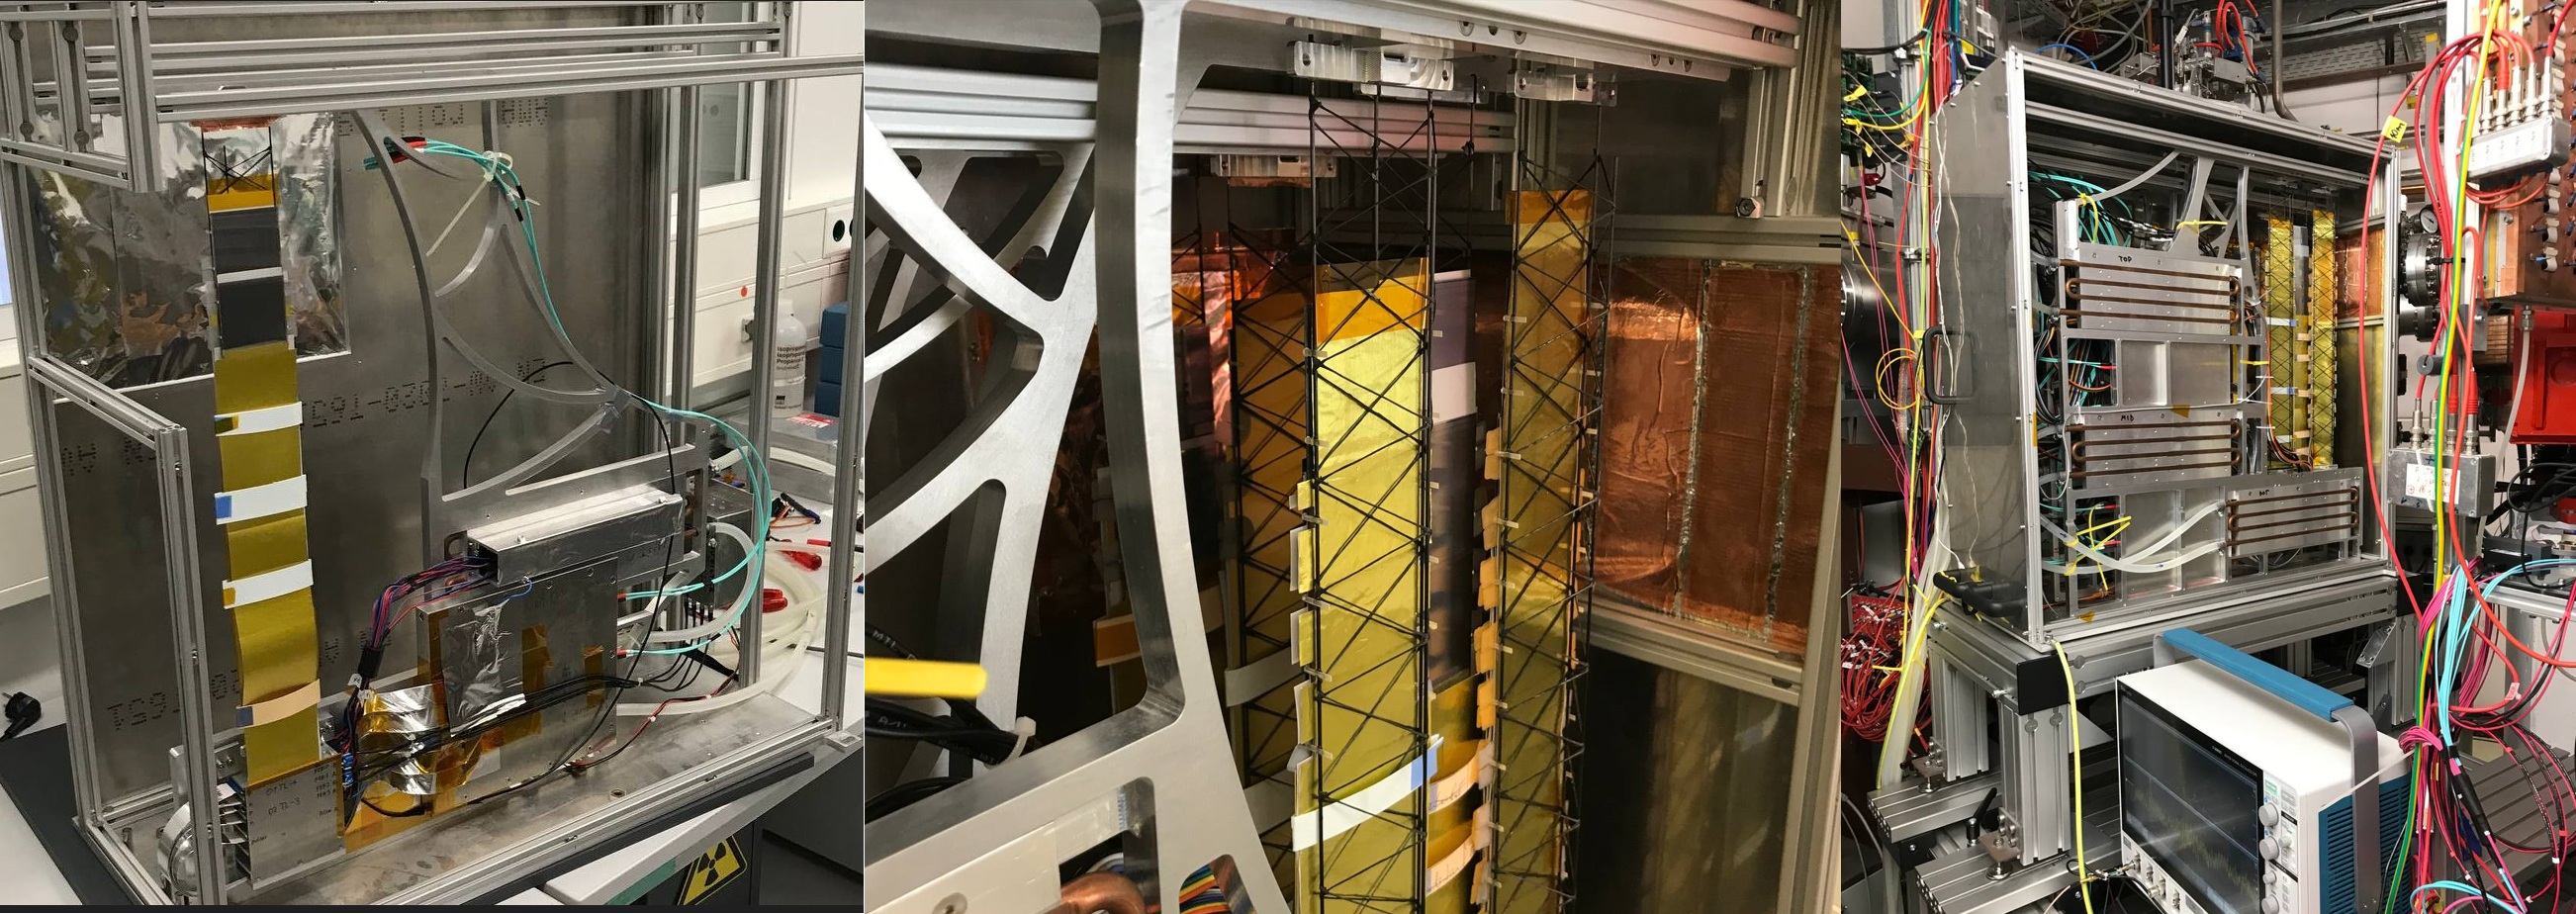
\includegraphics[width=0.99\columnwidth]{Chapter6/DCS/images/msts_all.png}
\caption{Assembly process of the \gls{mSTS} (from left to right)}
\label{fig_msts_state}
\end{figure}
%\newpage
 The first photo on the left side depicts the first c-frame after installing it inside the detector's enclosure. The second photo shows one of the last stages of the detector assembly, all detector modules are mounted. The last photo shows the detector after its transfer to the experiment cave and the last checks related to detector services. %\newpage

\section{Operation of the mSTS}

The \gls{mSTS}'s \gls{DCS} is a fairly automatized system in which monitoring and control are taken care of by the Finite State Machine. An operator, that is most likely the person tackling the data acquisition system, should monitor leakage current, temperatures, dew point, availability of the nodes as well as the overall system state (based on the \gls{FSM}). All the logs are available either in Phoebus or Kibana. Moreover, the alarm server together with Phoebus takes care of notifying the operator about alarms (exceeding limits, communication errors, etc.). This section contains the summary of the most important findings which were obtained through the \gls{DCS}. 
\subsection{Power dissipation of the mSTS}
 Power consumption of the 11 modules (22 \glspl{FEB}) of the \gls{mSTS} was studied in detail to better understand the differences between the modules and estimate how predictions meet the experimental results. The values obtained through the \gls{mSTS} were compared with the measurements of two frond-end boards and average values from modules calibration. In order to compare the results, the \gls{CSA} (front and back register) of all STS-XYTERs were changed to values from 7 to 42 with a step of 5.
 
 Figure \ref{fig_power_scheme} depicts the power dissipation of different components based on the \gls{CSA} value for measurements conducted with a separate pair of \gls{FEB}s. These two \glspl{FEB} were powered directly using a \gls{LV} power supply (R\&S~HMP4040). The power dissipation estimations for the distribution lines and the DC/DC converters were performed based on the assumed efficiency of 80 \%, which might be lower for $I > 2$~A dropping down to 65~\% at \SI{10}{\celsius} with currents approaching the device output limit (3~A). In this case, due to the settings of the \glspl{ASIC} the currents for the digital line were slightly higher than expected for the operation - around 2.3~A instead of 1.9~A. The analog line currents are defined by the \gls{CSA} register values and in this case varied from 1.4~A to 4.1~A.  Due to the experimental nature of the \gls{mSTS} and its powering scheme, the voltage drop of every element in the distribution lines can't be determined accurately. Therefore, the calculations made for the distribution lines based on the currents measured for the \glspl{FEB} and modules can't be considered as a reference. A detailed description of the powering scheme can be found in section~\ref{module}.  For this estimation, a constant value of voltage drop in the \gls{LDO} regulators of 0.6~V was assumed. 

 
\begin{figure}[h!]
\centering
\includegraphics[width=0.65\columnwidth]{Chapter6/DCS/images/POB.png}
\caption{mSTS's powering scheme with power dissipation estimations for different components depending of the \gls{CSA} value set}
\label{fig_power_scheme}
\end{figure}


The pie charts in the figure \ref{fig_power_CSA} show that while increasing the power consumption of the \gls{ASIC}s we also significantly increase the share of the power dissipated by the DC/DC converters and distribution lines. %\newpage
\newpage
\begin{figure}[h!]
\centering
\includegraphics[width=0.7\columnwidth]{Chapter6/DCS/images/POBpie.png}
\caption{Power dissipation share of different components of the powering scheme depending on the \gls{CSA} value}
\label{fig_power_CSA}
\end{figure}
Figure \ref{fig_power2} shows the current drawn by 4 \glspl{FEB} of unit 1 depending on the \gls{CSA} value. It was determined that the \gls{CSA} value of 31 should be the nominal value for the \gls{STS} modules, as it is a default value for the STS-XYTERv2.2 and this value also ensures that the signal amplification is correct (\gls{CSA} value of 31 corresponds to 2~mA per analog channel). Nevertheless, the \gls{CSA} value may vary to address the different needs of modules (depending for example on their noise levels).  Moreover, the DC/DC converter responsible for powering the analog front end (\gls{AFE}) is limited to the 3~A, therefore also the higher values of \gls{CSA} won't lead to higher current in the circuit.
%\begin{figure}[h!]
%\centering
%\includegraphics[width=0.45\columnwidth]{Chapter6/DCS/images/U0CSABIAS.png}
%\includegraphics[width=0.45\columnwidth]{Chapter6/DCS/images/U1CSABIAS.png}
%\caption{CSA scan of the unit 0 (left) and 1 (right)}
%\label{fig_power1}
%\end{figure}

\begin{figure}[h!]
\centering
\includegraphics[width=0.6\columnwidth]{Chapter6/DCS/images/U2CSABIAS.png}
\includegraphics[width=0.6\columnwidth]{Chapter6/DCS/images/U3L1CSABIAS.png}
\caption{CSA scan of the unit 2 (upper) and unit 3 ladder 0 (lower)}
\label{fig_power2}
\end{figure}
\newpage
Similar measurements were also conducted for all the other \gls{mSTS} modules (see Appendix~\ref{CSA}). The average values of the current (a module is powered by two low voltage channels) for every unit are depicted in the figure \ref{fig_avg}. For the older modules, especially those powered by 1.8 V and 2.4~V DC/DC converters (Unit 3), the currents are significantly higher, reaching 1.6 - 1.8~A for the \gls{CSA} 31. The \gls{AFE} of the unit 1 modules are powered by the 1.8~V \gls{LDO} regulators with a diode, which causes a voltage drop of approximately 0.6~V. Nevertheless, this sub-optimal solution can be also seen via increased current and power dissipation of the unit 1 modules. The current of modules of units 0 and 2 are similar, as they use the same components, which are also considered the final parts for the \gls{STS}.

%\newpage
\begin{figure}[h!]
\centering
\includegraphics[width=0.6\columnwidth]{Chapter6/DCS/images/units.png}
\caption{Average current of each \gls{mSTS} unit}
\label{fig_avg}
\end{figure}

The modules are powered in the constant voltage mode, which means that the output voltage is always 10.5~V. Knowing the currents at the power supply level, cable lengths, and voltage drops on subsequent components, the power estimation can be made based on the equation:
\begin{equation}
    P = VI
\end{equation}
Moreover, we can also try to estimate the power consumption based on the values from the module testing prior to the detector assembly. Average values of the currents are presented in the \ref{tab:typical_cons}. By adding estimates related to the distribution lines and DC/DC converters from figure~\ref{fig_power_scheme} we can compare the results with the \gls{mSTS} results. 
\begin{table}[!h]
\centering
\begin{tabular}{lll}
\hline
CSA & Current digital {[}A{]} & Current \gls{AFE} {[}A{]} \\ \hline
15  & 1.9                 & 1.02                    \\
31  & 1.9                 & 2.05                    \\
48  & 1.9                 & 3.07                    \\
63  & 1.9                 & 4.10                    \\ \hline
\end{tabular}
\caption{Currents supplied to the analog front end and to the digital part depending on the set \gls{CSA} value}
\label{tab:typical_cons}
\end{table}
\newpage
Figure \ref{fig_theor} shows the comparison of the power consumption of \gls{mSTS} units with the calculations based on the average current from the modules testing (depicted as FLA v2) and FEB currents (denoted as FLA). The values obtained from the calculation follow unit 1 power consumption. 

\begin{figure}[h!]
\centering
\includegraphics[width=0.65\columnwidth]{Chapter6/DCS/images/theor.png}
\caption{Average power dissipation of the units compared with predictions based on theoretical power dissipation in the components (depicted as FLA)} 
\label{fig_theor}
\end{figure}
The components used for units 0 and 2 are considered to be almost the final ones, therefore the power consumption of these modules should serve as a reference for further calculations. Some parameters related to the voltage drop may change, mostly due to different powering lines' lengths and diameters, as well as different connectors. 
\begin{table}[h!]
\centering
\begin{tabular}{lll}
\hline
               & \gls{CSA} 31  & \gls{CSA} 48  \\ \hline
FLA estimation & 31.5 kW & 38.8 kW \\
Unit 3         & 32.9 kW & 41.3 kW \\
Unit 2         & 24.7 kW & 29.9 kW \\ \hline
\end{tabular}
\caption{Total power consumption of the 876 modules of the \gls{STS} based on the calculations from the figure~\ref{fig_theor}}
\label{tab:power_cons}
\end{table}
Therefore, the values stated in the table~\ref{tab:power_cons} can't be considered as a reference. Nevertheless, they give a good estimation of the power consumption and also show how the module assembly evolved. 
%\newpage
\subsection{Parameters monitoring and obtained data}
All the software and hardware components mentioned in the previous sections deliver essential information about the detector's safety and health. Thanks to the ongoing ambient monitoring many features of the subsystem were discovered and addressed, e.g. not sufficient cooling. Figure \ref{fig_temp} shows the temperature trends during the 450 days of operation. The first sensor (depicted in blue) was placed at the top of the \gls{mSTS}'s enclosure, and the second one (depicted in orange) is located on the upper part of unit 2. Temperatures registered in the \gls{mSTS} vary not only depending on the \gls{FEE} powering (peaks observed throughout the period) but also on the temperature in the cave. Moreover, the broader peak at the end of the depicted period is associated with the cooling unit's failure.  There are also a few periods, with the longest in December and January, when the detector was not operated. 

\begin{figure}[!h]
\centering
\includegraphics[width=0.55\columnwidth]{Chapter6/DCS/images/temp2.png}
\caption{Temperature monitoring}
\label{fig_temp}
\end{figure}

To ensure the safe operation of the system, it's also necessary to have information about the dew point. Water condensation on the parts of the \gls{FEE} could cause a whole ladder to fail. Figure \ref{fig_dew} depicts the differences in the dew point and temperature over the mentioned period. The coolant setpoint was always carefully adjusted depending on the situation in the experiment cave. 
\newpage
\begin{figure}[!h]
\centering
\includegraphics[width=0.55\columnwidth]{Chapter6/DCS/images/dew.png}
\caption{Temperature and dew point monitoring}
\label{fig_dew}
\end{figure}


Apart from ambient temperature and humidity monitoring, temperature sensors are also used to monitor the temperature on the powering boards. A comparison of the temperature on the \gls{POB} of unit 1, 2 and between two POBs of unit 3 are presented in the figure~\ref{fig_POB1}. Temperature measured in the unit 3, especially at the beginning of the operation, were much higher than those measured in unit 0 and 1. This effect is associated with a cooling issue which was resolved at the beginning of 2022. At the right end of the plot, we can see again the cooling unit failure. 
\begin{figure}[!h]
\centering
\includegraphics[width=0.55\columnwidth]{Chapter6/DCS/images/POB1.png}
\caption{Temperature on the POBs enclosure}
\label{fig_POB1}
\end{figure}
\newpage
Moreover, the temperature on the \gls{ROB} and \gls{FEB} was monitored, as depicted in the figure~\ref{fig_robvsfeb}. Interestingly, the temperature on the \gls{ROB} is higher than the temperature on the \gls{FEB} box on the unit 2. Unit 2 features 2 modules, 4 \gls{FEB}s (+ pulser board) in the \gls{FEB} box (each drawing about 1.6 A at constant 10.5 V), in comparison to the \gls{ROB} which is powered with 7 V and consumes about 0.8 A. This is, most likely, related to the position of better contact of the \gls{FEB} box to the cooling plate.

\begin{figure}[!h]
\centering
\includegraphics[width=0.55\columnwidth]{Chapter6/DCS/images/ROBvsFEB.png}
\caption{Temperature on the \gls{ROB}, \gls{FEB} box}
\label{fig_robvsfeb}
\end{figure}

\subsection{Monitoring of the leakage current}

Information about the temperatures serves not only to ensure detector safety but also to understand the behavior of the silicon sensors properly. Especially when analyzing and comparing the leakage current of the sensors, the temperature is of high importance as it allows the normalizing of the current to the same value. Firstly, if the exact temperature characteristic of the sensors is now known, it's necessary to rely on a temperature sensor placed close to the semiconductor. In the \gls{mSTS} several sensors are measuring ambient conditions, an overview can be seen in figure \ref{fig_temperatures}. The temperature inside the detector is significantly lower, which indicates that the cooling is working. Higher temperatures are also seen on the top of the detector. 

\newpage
\begin{figure}[!h]
\centering
\includegraphics[width=0.55\columnwidth]{Chapter6/DCS/images/rates/tempmSTS.png}
\caption{Distributions of the temperatures inside the \gls{mSTS}}
\label{fig_temperatures}
\end{figure}

As the silicon sensors are reverse-biased, the nominal operating voltage was chosen to be $\pm75$ (as the full depletion of the non-irradiated silicon sensors is assured). The reverse polarity implies also negative current values. Nevertheless, only one side or channel will be discussed. The other side of the sensor is characterized by the same trends, but opposite sign.

%\newpage
\begin{figure}[!h]
\centering
\includegraphics[width=0.45\columnwidth]{Chapter6/DCS/images/uranium/U0.png}
\includegraphics[width=0.45\columnwidth]{Chapter6/DCS/images/uranium/U3.png}
\caption{Leakage current of the silicon sensors in modules of units 0 and 3 during collisions of uranium with the gold target of different thicknesses.}
\label{fig_msts_LC}
\end{figure}

Typical behavior of the \gls{STS} silicon sensors during data-taking can be seen in figure~\ref{fig_msts_LC}. Due to radiation-induced surface and bulk damage, the leakage current will increase with the increasing total fluence that the sensors were exposed to. In order to properly compare the leakage current before and after the irradiation it's necessary to have the same ambient conditions or to measure the temperature and then normalize the current to \SI{20}{\celsius}. Apart from the constant leakage current rise during the data-taking, two particular parts of the plot can be distinguished. The first one just after 500 minutes when increased beam intensity leads to disclosing the spill structure. A similar trend can also be observed from around 1500 min until the end. The sensors of different units behave differently, depending on their position relative to the beam or sensor size, electrical short circuits.


\begin{figure}[!h]
\centering
\includegraphics[width=0.45\columnwidth]{Chapter6/DCS/images/uranium/current_U_highintensity.png}
\includegraphics[width=0.47\columnwidth]{Chapter6/DCS/images/uranium/U3L1_spill.png}
\caption{Unit 0 \gls{FEB} 3 - normalization of the current (left) and zoomed-in view of the spill structure seen by the silicon sensors (10 s spill)}
\label{fig_sensors_spill}
\end{figure}

An example of the normalization of the unit 1 sensors is depicted in the figure~\ref{fig_sensors_spill}. A more detailed view of the spill structure is shown on the right plot. It can be clearly seen, that the reaction products traversing the silicons cause a significant leakage current increase of about \SI{10}{\micro A} (for the highest beam intensities - $10^{9}$ ions/s). Comparison of two units leakage current which was scaled to $20\,^{\circ}$C is shown in figure \ref{fig_leak}. Throughout the year 2021, only a few beam time campaigns took place, therefore leakage current increase due to radiation-induced damage is negligible. On the other hand, during the beam campaigns of 2022, the effect of radiation can be clearly seen.

\begin{figure}[!h]
\centering
\includegraphics[width=0.45\columnwidth]{Chapter6/DCS/images/sensors/U0_leakage.png}
\includegraphics[width=0.45\columnwidth]{Chapter6/DCS/images/sensors/U3_leakage.png}
\caption{Leakage current evolution of the \gls{mSTS} sensors over the whole period of operation}
\label{fig_leak}
\end{figure}

\newpage
The quantitative current changes over the \gls{mCBM} campaign are shown in the table~\ref{tab:msts_final_fluence}. To better understand the overall results, it's important to take a look at the position of the silicon sensors with respect to the beam (see~figure~\ref{fig_sensors_scheme}). The sensors located closer to the collision point (from unit 0) are more irradiated than sensors from units 2 and 3. Furthermore, the results obtained from unit 3 are inconsistent throughout the experiment, which means that those modules are considered to have electrical issues (e.g. short circuits).


\begin{table}[!h]
\centering
\begin{tabular}{lcc}
\multicolumn{1}{c}{Module} & \begin{tabular}[c]{@{}c@{}}Current \\ difference {[}uA{]}\end{tabular} & Fluence {[}n/cm2{]} \\ \hline
U3L1M0                     & 16.23                                                                  & $2.5*10^{11}$          \\
U3L1M1                     & 7.6                                                                    & $5.8*10^{10}$          \\ \hline
U3L0M0                     & 3.7                                                                    & $5.7*10^{10}$          \\
U3L0M1                     & 4.1                                                                    & $6.2*10^{10}$          \\
U3L0M2                     & 3.5                                                                    & $5.3*10^{10}$          \\ \hline
U2M0                       & 3.6                                                                    & $5.5*10^{10}$          \\
U2M1                       & 6.3                                                                    & $4.8*10^{10}$          \\ \hline
U1M0                       & 6.4                                                                    & $9.8*10^{10}$          \\
U1M1                       & 6                                                                      & $9.1*10^{10}$          \\ \hline
U0M0                       & 6.9                                                                    & $1.1*10^{11}$          \\
U0M1                       & 7.2                                                                    & $1.1*10^{11}$         
\end{tabular}
\caption{Leakage current differences and corresponding fluence estimations for all the \gls{mSTS} modules.}
\label{tab:msts_final_fluence}
\end{table}

\begin{figure}[!h]
\centering
\includegraphics[width=0.4\columnwidth]{Chapter6/DCS/images/msts_sensors_scheme.png}
\caption{Schematic view of the \gls{mSTS} sensors position with respect to the beam}
\label{fig_sensors_scheme}
\end{figure}
\newpage
\subsection{IV characteristic of chosen modules}
The IV curves provide crucial information about the detector performance (see section \ref{sensors}):
\begin{itemize}
    \item shot noise, closely related to the leakage current which increases with the fluence,
    \item type inversion,
    \item annealing and reverse annealing,
\end{itemize}
Figure \ref{fig_IV} shows IV curves of two modules from two different units (1 and 3). 
\begin{figure}[!h]
\centering
\includegraphics[width=0.45\columnwidth]{Chapter6/DCS/images/IV/U0FEB1.png}
\includegraphics[width=0.45\columnwidth]{Chapter6/DCS/images/IV/U3L1FEB1.png}
\caption{IV curves for two modules from different units}
\label{fig_IV}
\end{figure}

The leakage current is scaled down to $\SI{20}{\celsius}$ but the relative humidity was different for each measurement. The IV measured during the QA procedure before the assembly of the module is depicted in yellow and shows a typical behavior of a revers-biased silicon diode with a full depletion reached around 60-70~V. The two other IV measurements for each module took place after assembly in the \gls{mSTS}, the beam campaign with the uranium beam, and the end of data-taking for 2022. The linear behavior of the sensors can be seen after the module assembly, measuring with an external high-voltage filter in a floating scheme. Nevertheless, the unit 3 sensor shows breakdown at similar biasing voltage for all three measurements. Figure~\ref{fig_IV_good} shows the IV measurement of a module without additional \gls{HV} filter and a Keithley power supply instead of Wiener \gls{LV} module. The \gls{HV} filter was integrated in the new version of the \gls{FEB} (FEB8-3), therefore new measurements will take place to establish the behavior of the module with the new PCB.

\begin{figure}[!h]
\centering
\includegraphics[width=0.5\columnwidth]{Chapter6/DCS/images/IV/30304Whole.png}
\caption{IV curves of a module}
\label{fig_IV_good}
\end{figure}

\newpage
\subsection{Data rates and leakage current}
Data rates from subsystems contain important information about the detector performance. Figure~\ref{fig_data_rates_Ag} shows an example of the \gls{mSTS} operation during data-taking with \footnote{gold beam colliding with gold target}{Au+Au} system ($T= 1~\mathrm{AGeV}$) and later with Ni+Ni system (without the \gls{mSTS}). Data rates are clearly correlated with the beam intensity. Regardless of the beam intensities, the \gls{mSTS} (with the chosen settings) is responsible for more than half of the total data. During the beam intensities of $10^{8}$ ions/s, \gls{mSTS}'s data rate was about 500 MB/s and with the maximum beam intensities it was up to 2000 MB/s, reaching the limits \gls{FEB}s uplink. 
\begin{figure}[H]
\centering
\includegraphics[width=0.55\columnwidth]{Chapter6/DCS/images/rates/Ag_total.png}
\caption{Data rates of all the \gls{mSTS} units in comparison to the overall data rate of all subsystems during data-taking}
\label{fig_data_rates_Ag}
\end{figure}
\newpage
There is a direct correlation of data rates with the leakage current increase, what can be seen in figure~\ref{fig_Data}. This correlation gives more insight into the operation and state of the silicon sensors.
\begin{figure}[!h]
\centering
\includegraphics[width=0.45\columnwidth]{Chapter6/DCS/images/U1_data_rate.png}
\includegraphics[width=0.45\columnwidth]{Chapter6/DCS/images/U2_data_rate.png}
\caption{Leakage current evolution of the \gls{mSTS} silicon sensors and respective integrated data rate}
\label{fig_Data}
\end{figure}

\section{Conclusions}

The successful operation of the \gls{mSTS}, including the \gls{DCS} and \gls{DAQ} chain set an important milestone toward completion of the \gls{STS} project. The first extensive data-taking activities with two tracking stations proved the general idea behind the assembly of the detector. The prototyping of the supervisory layer of the \gls{mSTS} detector took place and was successfully concluded, proving that the concept was extremely useful, not only for a large detector, accelerator setups but also for smaller experiments. After almost two years of operation of the containers based system proved to be a reliable, easily maintained solution. Nevertheless, for the final system, several additional applications are needed. The \gls{STS} will be much more complex and challenging when it comes to configuration and running. Moreover, it will be extremely important to have both hardware and software interlocking to ensure the machine's safety.

The \gls{mSTS} didn't publish its overall status to any external agent. Due to that reason, some information like \gls{ASIC} internal temperature or $V_{DDM}$ were only accessible via the data acquisition chain (\gls{DCA}-\gls{CRI}). In the future, each subsystem will have an assigned \gls{SCA} to tackle control of the readout chain and the \gls{DCS}. 


Temperature sensors located inside the \gls{mSTS} and information about the current drawn by the sensors indicate the silicon sensors' state. The sensors may degrade over time due to radiation-related bulk damage,  which leads i.a. to leakage current increase, type inversion, etc. Those effects can be partially studied through the \gls{DCS} and the control strategy adopted respectively to the results.

Figure \ref{fig_dcs_results} shows the how the \gls{DCS} performed during about 2 years of operation. Due to the radiation-induced soft errors in the controllers of the cooling units, there were several occasions that the operation of the \gls{STS} needed to be halted. Usually, such an interruption in the operation was automatically triggered by the \gls{FSM}. Nevertheless, listed errors might also include the intervention in the system. In that case the error related to the cooling system was logged, but the FSM might have been off.
\begin{figure}[!h]
\centering
\includegraphics[width=0.55\columnwidth]{Chapter6/DCS/images/DCSpie.png}
\caption{Results from the operation}
\label{fig_dcs_results}
\end{figure}



%\subsection{Experiment overview and its goals}
%\subsection{Prototyping of the DCS based on the mSTS}
%\subsection{Design and functionalities of the DCS}
%\subsection{Silicon sensors' leakage current monitoring}
%\section{Monitoring of the Front End Electronics' parameters}

%\section{Applications of the control software}
%\subsection{Control and monitoring of a custom climatic chamber for studies of thermal interfaces}


%\chapter{Solutions for humidity and temperature monitoring in the STS}
\chapter{Solutions for humidity and temperature monitoring in the STS}
The design of the \gls{STS} \cite{Heuser:54798} defines the requirements for ambient sensors. As described in the section~\ref{cooling}, the ambient temperature will reach \SI{-10}{\celsius} at the end of the \gls{STS} lifetime. The cooling liquid (3M NOVEC 649) will be circulating at temperatures close to \SI{-40}{\celsius}. Therefore, the first boundary condition arises - the frost point needs to be below \SI{-40}{\celsius} to avoid ice formation or condensation on the \gls{FEE}. For the first few years of operation, the temperatures will be higher and therefore RH/frost point can be measured more accurately. One of the most common techniques to achieve the frost points below \SI{-40}{\celsius} is baking. In the case of the silicon tracker, too high temperatures could destroy the \gls{FEE}. 
During the detector's lifetime (10 years), there will be only limited opportunities to do any upgrades. Therefore, the sensors have to withstand the radiation accumulated during that period. As some of the sensors can be placed in the vicinity of the beam pipe, the total dose could reach more than 10~kGy. The humidity measurements will take place in a distributed fashion, implying that different sensors may face different doses. As the detector will be placed in a dipole magnet providing a magnetic field of \SI{1}{\tesla\metre}, the sensors need to be insensitive to it. An ideal humidity sensor should meet the following requirements:
\begin{itemize}
    \item small dimensions and mass (especially when placed close to the active area of the system),
    \item accurate relative humidity readouts at temperatures down to \SI{-20}{\celsius}, 
    \item ideally respond to a wide range of \gls{RH} values from 0~\% to 80~\%,
    \item high repeatability and low hysteresis,
    \item reliable operation across long distances (the readout device needs to reside at least \SI{20}{\metre} away from the detector).
\end{itemize}

\section{Introduction to humidity measurements}


$DP(T, RH) = \frac{\lambda(ln(\frac{RH}{100})+\frac{\beta T}{\lambda + T})}{\beta - (ln(\frac{RH}{100})+\frac{\beta T}{\lambda + T}}$

\section{Overview of different technologies}
In a constraint volume of the 
\section{Motivation and market availability of different sensor types}

\subsection{Capacitive sensors}

\subsection{Fiber optic sensors}

\subsection{Dew point transmitters}


\section{Fiber Bragg Grating technology}

Fiber Bragg Grating is a type of selective filter that reflects light signals at a specific wavelength known as the Bragg wavelength (see Figure 1). A bare FBG inscribed into the fiber core is temperature and strain sensitive.
We can measure RH instead of strain by applying a hygroscopic material (for example, polyimide) to the cladding. The Bragg wavelength shift becomes a superposition of temperature and humidity effects in this case (see equation (see equation \ref{eqn:FBG}) \cite{Kronenberg:02}. 
                            %\newpage
                             \begin{equation}\label{eqn:FBG}
                            %\large
                                    \frac{\Delta\lambda_{B}}{\lambda_{B}}=\Delta TS_{T}+\Delta RHS_{RH}
                            \end{equation}
                            $\lambda_{B}$ - Bragg wavelength, $S_{RH/T}$ - sensitivity  coefficients for RH and temperature, respectively. \newline
In order to measure RH, it’s crucial to have precise temperature readouts in the vicinity of the coated FBG. Otherwise, the actual RH readout may be dominated by uncertainty or just the inaccurate temperature measurement.

\begin{figure}[!h]
\centering
\includegraphics[width=0.4\columnwidth]{Chapter4/Images/Picture1.png}
\caption{Hygrometer (Temperature and humidity sensitive FBG inscribed into the same fiber)}
\label{fig_single_photo}
\end{figure}
\section{Evaluation and measurement setup}
A few different humidity sensors have been tested and their performance evaluated. Use of capacitive sensors remains one of the cheapest and easily available solutions for a distributed humidity measurement system. 


\section{Results}


\subsection{Characterization of RH FOS}

\begin{figure}[!h]
\centering
\includegraphics[width=0.65\columnwidth]{Chapter4/Images/single1.jpeg}
\caption{Hygrometer (temperature and humidity sensitive FBG inscribed into the same fiber)}
\label{fig_single_photo}
\end{figure}

\begin{figure}[!h]
\centering
\includegraphics[width=0.6\columnwidth]{Chapter4/Images/rh.png}
\caption{Humidity induced Bragg wavelength shift for the single RH+T sensor}
\label{fig_single_wavelength}
\end{figure}


\begin{figure}[!h]
\centering
\includegraphics[width=0.6\columnwidth]{Chapter4/Images/rh.png}
\caption{Humidity induced Bragg wavelength shift for the hygrometer}
\label{fig_single_wavelength}
\end{figure}


\begin{figure}[!h]
\centering
\includegraphics[width=0.6\columnwidth]{Chapter4/Images/hygr.png}
\caption{Hysteresis}
\label{fig_hygrometer1}
\end{figure}


\begin{figure}[!h]
\centering
\includegraphics[width=0.6\columnwidth]{Chapter4/Images/RHS.png}
\caption{Calibration curves for the hygrometer}
\label{fig_single_calibration}
\end{figure}


\begin{figure}[!h]
\centering
\includegraphics[width=0.6\columnwidth]{Chapter4/Images/rh_array2.png}
\caption{Humidity induced Bragg wavelength shift for the sensors array}
\label{fig_single_calibration}
\end{figure}

\subsection{Calibration}

\begin{figure}[!h]
\centering
\includegraphics[width=0.6\columnwidth]{Chapter4/Images/comp.png}
\caption{Hysteresis}
\label{fig_calibration}
\end{figure}


\begin{figure}[!h]
\centering
\includegraphics[width=0.6\columnwidth]{Chapter4/Images/comp1.png}
\caption{Hysteresis}
\label{fig_calibration1}
\end{figure}





\subsection{Time response}

\begin{figure}[!h]
\centering
\includegraphics[width=0.6\columnwidth]{Chapter4/Images/20responseRH.png}
\caption{Time response of sensors}
\label{fig_time_response}
\end{figure}

\begin{figure}[!h]
\centering
\includegraphics[width=0.6\columnwidth]{Chapter4/Images/20responseRH.png}
\caption{Time response of sensors}
\label{fig_time_response}
\end{figure}


\subsection{Hysteresis}

\begin{figure}[!h]
\centering
\includegraphics[width=0.6\columnwidth]{Chapter4/Images/25_RHS.png}
\caption{Hysteresis}
\label{fig_hysteresis}
\end{figure}

\begin{figure}[!h]
\centering
\includegraphics[width=0.6\columnwidth]{Chapter4/Images/25_RHST.png}
\caption{Hysteresis}
\label{fig_hysteresis2}
\end{figure}



\subsection{Repeatability}


\begin{figure}[!h]
\centering
\includegraphics[width=0.6\columnwidth]{Chapter4/Images/repeat.png}
\caption{Repeatability}
\label{fig_repeatability}
\end{figure}



\subsection{Conclusions}


\begin{figure}[!h]
\centering
\includegraphics[width=0.6\columnwidth]{Chapter4/Images/DPCPercent.png}
\caption{Comparison}
\label{fig_comparison}
\end{figure}

\begin{figure}[!h]
\centering
\includegraphics[width=0.6\columnwidth]{Chapter4/Images/FOS_performance.png}
\includegraphics[width=0.6\columnwidth]{Chapter4/Images/FOS_performance_T.png}
\caption{Comparison}
\label{fig_comparison}
\end{figure}

\subsection{Conclusions}
The total uncertainty of the hygrometer obtained after including the calibration error and the hysteresis is $1.7$\%RH. For the array sensors, the uncertainty is about $4\%$.
As the hygrometer design turned out to be more consistent and robust, it was also tested with the sniffing system and its ceramic sensor. The sensors array didn't provide the expected repeatability and it needs will be further tested inside the thermal demonstrator (see section~\ref{demo}). The design and the performance of the hygrometer were confirmed during the low-temperature tests with the industrial capacitive sensors and with the trace humidity sensor (see figure~\ref{fig_comparison}). The uncertainties of the sensors were not shown, in order to represent the trends of the respective sensors. The largest uncertainty is associated with the capacitive sensor. 
\begin{figure}[!h]
\centering
\includegraphics[width=0.6\columnwidth]{Chapter5/images/DPCPercent.png}
\caption{Comparison of the dew points calculated using the Magnus formula for the industrial sensor SHT85, metal oxide trace humidity sensor, and the hygrometer. For the comparison, the temperature inside the Binder climatic chamber was also plotted.}
\label{fig_comparison}
\end{figure}
The response of the hygrometer was also compared with the sniffing system and different lengths of the guidelines leading to the ceramic sensor. In the case of the \gls{STS} the sniffing system's electronic circuitry will be placed at least \SI{20}{\metre} away from the detector. For the plot depicted on the left side, the pipe was \SI{2}{\metre} and for the right one \SI{12}{\metre}, the time response was $1.5$~min and $3$~m. Assuming that the flow doesn't depend on the distance from the sniffing point if the pipe was $30$~m the response would be $5.7$~min. 
\begin{figure}[!h]
\centering
\includegraphics[width=0.47\columnwidth]{Chapter5/images/DPCPercent_response2m.png}
\includegraphics[width=0.47\columnwidth]{Chapter5/images/DPCPercent_response12m.png}
\caption{Time response comparison of different sensors. Left - \SI{2}{\metre} pipe to the ceramic sensors, right - \SI{12}{\metre} pipe to the ceramic sensors.}
\label{fig_comparison}
\end{figure}
\newpage
Figure \ref{Tfig_comparison_2} shows the behavior of the fiber optic hygrometer at low dew points. The sensing limits are clearly represented in the figure~\ref{Tfig_comparison_2} with a red rectangle. Considering the area with a high point density, the limitations of the hygrometer could be assumed to be a dew point of \SI{-70}{\celsius}. But in that area, the uncertainties become much higher. It's also noteworthy that that limit refers to the measuring temperature of \SI{10}{\celsius}. On the other hand, for the dew points measured at \SI{20}{\celsius} the range shrinks to values of about \SI{-50}{\celsius}/\SI{-40}{\celsius}.

\begin{figure}[!h]
\centering
\includegraphics[width=0.47\columnwidth]{Chapter5/images/FOS_performance_T.png}
\includegraphics[width=0.47\columnwidth]{Chapter5/images/FOS_performance1.png}
\caption{The temperature inside the BINDER chamber and temperature measured by the hygrometer(left). Dew point during the changing ambient conditions per the hygrometer and the ceramic sensor.}
\label{Tfig_comparison_2}
\end{figure}
\section{Final considerations}
The characterization of the \gls{FOS} pointed out the advantages and limits of this particular technology with the use of polyimide as the sensitive material. In principle, the tested hygrometer meets the requirements set for the \gls{STS}. The distributed system could be also based on the \gls{FOS}. An array of sensors could be still considered, but the distance between the gratings should be much larger than \SI{15}{\cm} to ensure that the sensors can be put inside packaging in strain-free conditions. As mentioned in the section~\ref{fos_irrad}, the \gls{FBG} based \gls{FOS} can be considered radiation hard. According to Berutti~\cite{Berruti}, the sensors can be used in radiation environments by pre-irradiating them before installation, to reduce radiation-induced cross-sensitivity. 

Moreover, the capacitive industrial sensors will be used next to the \gls{FOS}. The main purpose will be to use them during the commissioning and in order to recalibrate the \gls{FOS} if the installation will cause any additional stress on the grating.

The last technology foreseen for the distributed sensing system is the metal oxide moisture sensor, which is a very reliable solution that will be used also for the interlocking system.  Several sniffing points inside the detector enclosure will also measure trace humidity and serve as a reference for the two other measurement technologies.

%\section{Overview of different technologies}
%\section{Motivation and market availability of different types of sensors}
%\subsection{Capacitive sensors}
%\subsection{Fiber Optic sensors}
%\subsection{Dew point transmitters}
%\section{Fiber optic sensing technology}
%\section{Fiber Bragg Grating technology for humidity and temperature monitoring}
%\section{Evaluation and choice of the measurement setup}
%\section{Characterization of the RH FOS}
%\section{Time response and uncertainty of the FOS}
%\section{Hysteresis}
%\section{Conclusions}


\chapter{On the way to the Silicon Tracking System}
\section{Thermal Demonstrator and its controls}
\subsection{Setup overview and its goals}
\subsection{Controls overview}
\subsection{Outlook for the DCS software services} 
Software applications introduced in the thesis proved to be extremely useful for small and medium size setups (up to a few thousand \glspl{PV}. Nevertheless, for the final experiment, a more sophisticated software infrastructure is needed.

The final system will feature an orchestrator which should be scalable, highly available, provide logging, and monitoring capabilities, and be redundant. Orchestration leads to automation of the container deployment, as well as to balance the workload. Orchestrators can:
 \begin{itemize}
     \item Automatically deploy containers based on policies, application load, and environmental metrics.
     \item Identify failed containers or clusters and heal them.
     \item Manage application configuration.
     \item Connect containers to storage and manage networking.
     \item Improve security by restricting access between containers, and between containers and external systems.
 \end{itemize}

 Examples of orchestrators include DockerSwarm~\cite{DockerSwarm}, and Kubernetes \cite{Kubernetes}. One of the recent applications of Kubernetes was reported in \cite{ICALEPCS2021:Diamond}, where the whole test beam line is operated with containers. Similarly, the whole \gls{CBM} \gls{DCS} could be operated with containers and orchestration tools. 

 Apart from the orchestration, the \gls{DCS} should be supplemented with:
 \begin{itemize}
      \item Gateway(s) - considering the low voltage powering of the \gls{STS} \gls{FEE}, which consists of about 2100 low voltage channels, 140 modules, and 14 crates. Each crate has a controller with an embedded \gls{IOC}, publishing all the process variables. By putting the power supplies into a different subnet or network, it is possible toe easily debug potential problems and limit the network traffic. That is why it has been endorsed to use CA Gateway \cite{gateway} or \gls{PV} gateway, which will take care of regulating access between the subnets in the DCS network. It also provides additional access security, assuring that the \glspl{IOC} running the key services like powering run smoothly.
     \item Time synchronization - as mentioned in Section \ref{archiver}, the archiver could be split into a few nodes serving as temporary data storage (short-term, mid-term). Proper daily backup to GSI managed database would be recommended, but it depends mostly on the database services provided by the GSI IT. So far, the Redis DB has been used, but also other options should be considered.       
     \item Logbook - one of the missing elements in the \gls{mSTS} architecture is a logbook. So far, for all the mCBM-related activities, elog \cite{elog} was used. For the final experiment, a dedicated elog branch will be implemented and the elog client will be used \cite{elog_client},
     \item Save and restore service - it is organized twofold. A tool, called autosave, which is a part of the synApps module \cite{autosave} preserves \glspl{PV} values through the \gls{IOC} reboot. The second set of tools that permits taking snapshots and saving configurations is MASAR \cite{masar}. It is a more complex tool than autosave, offering also a Phoebus-based \gls{GUI}.
     \item Data persistence - to properly archive and analyze the data, it is necessary that all nodes, \glspl{IOC}, and other software applications are synchronized. As it is impossible to adjust the clock in the containers, it should be synchronized on each node separately. The central \gls{DCS} node will provide a Network Time Protocol (\gls{NTP}) daemon that will be synchronized with one of the public, official sources.  By doing so, the clocks of all the containers running control applications will be automatically synchronized even if the external network connection is not available.
     \item Communication protocol - it was reported during the EPICS Collaboration meeting 2022 \cite{epics_2022} that the transition to the newer protocol (PV access) is ongoing. Nevertheless, CA and PVA are both included in the EPICS 7, which should be the base image of the \gls{CBM} \gls{IOC} image, and also for the next versions of the \gls{IOC}. PVA is under constant development and will offer even more features in the coming years, thus for the future CBM experiment (timeline of more than 10 years), it is an optimal choice. 
 \end{itemize}


\subsection{Failover considerations}
The high availability of services plays a key role in the safe operation of a detector. Once all the services are deployed, only short breaks are foreseen during 10 years of operation. The STS has to be constantly cooled, in order to avoid performance degradation of the silicon sensors and \gls{FEE}.

Crucial elements of the STS, like the air drying plant or the cooling plant, will be monitored and controlled by a \gls{PLC}-based system. This hardware layer will provide essential safety measures in case of failure. The \gls{PLC} will also be linked to an \gls{IOC} publishing the values to the software layer. 

Even before triggering the hardware interlock, any potentially hazardous system behavior will be discovered by the software of the control system. In order to ensure maximum safety, failover mechanisms will be exercised to mitigate potential \gls{IOC} failures. There are two considered methods to address failover:
\begin{enumerate}
    \item Considering a scenario in which the hardware is controlled, e.g., via a network. In that case, it is possible to deploy a backup \gls{IOC}, which has the same configuration as the main \gls{IOC}, therefore providing a replacement if it fails. Under some standards, like example RS232, it is not considered good practice to have two \glspl{IOC} connected to the same node. Furthermore, in the case of RS232 a multiplexer would be needed to implement a redundant solution. 
    \item A second possibility is to use failover mechanisms based on an orchestrator, in this case, the deployment and life cycle of a container is governed by an additional tool, i.e., Kubernetes. In case one of the containers (\glspl{IOC}) hangs up, it will be automatically stopped, and a new container will take over the tasks. Nevertheless, the newly deployed container could have a different configuration, therefore changing the state of the whole system. 
\end{enumerate}




%\section{Failure considerations}

%Failure considerations are an essential aspect of designing a detector and its services. Some systems might need to be planned as redundant structures that automatically bring a detector into a safe state in case of an issue and/or failure. For \gls{STS} there will be a few layers of dependencies and interlocks, including the software and hardware ones.

%Low voltage power supply failures can be divided into channel, module, controller, or crate failures. The example below describes the worst-case scenario in which the failed low-voltage module was connected only to the readout boards.
%\begin{itemize}
%    \item channel failure - in case of a permanent failure, up to 5 %\glspl{FEB} might be off (if that channel powers a \gls{ROB}),
%    \item module failure - up to 75 \glspl{FEB} might get disabled (4.3\% %of all boards), 
%    \item crate failure (10 \gls{LV} modules in the crate) - up to 750 %boards stop working, which constitutes to about 43\% of the STS.
%\end{itemize}

%As the LV power supplies will be located in the array which is not accessible during the beam time, any kind of permanent failure will result in a loss of the physics data. 

%Another type of failure that is dangerous for the system is an uncontrolled increase of water content inside the detector. This could be caused by the failure of the drying system, loss of confinement, or cooling system failure. 
%\section{Detector safety}


\section{Final remarks}

The scope of the thesis focused on developing a modular control system framework that can be implemented for small, medium, and large experimental setups. This framework was used for setups that required a remote operation, like the irradiation of the powering modules for the \gls{FEE}, but also in laboratory-based setups where the automation and archiving were needed (thermal cycling of the \gls{STS} electronics).

With the help of the \gls{EPICS} related applications, it was found that the low voltage powering module will experience soft errors of up to 9 per month during the \gls{CBM} operation. Such behavior poses a risk to the experiment operation as it could cause deterioration of the physics performance, but also a possible danger to the \gls{FEE}. On the other hand, the \gls{HV} channels would be switched off even more often, but in the case of the \gls{CBM} they are located far away from the experimental site.

It was further assessed what are the limitations of the \glspl{FEB} with respect to the thermal cycling and the mechanical stress that is therefore induced. The results served as an indication of possible failure modes of the \gls{FEB} at the end of \gls{STS} lifetime. Failure modes after repeated cycles, and potential reasons were determined (e.g., \gls{CTE} difference between the materials). 

Another application of the developed framework was related to the testing and characterization of the humidity sensors. A general strategy for ambient parameters monitoring inside the \gls{STS} was developed, and potential sensor candidates were chosen. A sampling system with a ceramic sensor and \gls{FOS} were identified as reliable solutions for the distributed sensing system. Additionally, the industrial capacitive sensors will be used as a reference during the commissioning.

The \gls{FOS} hygrometer turned out to be a more reliable solution in comparison to a sensor array. One of the possible reasons of  worse performance is a relatively low distance between the subsequent sensors and a thicker coating. The results obtained from the time response study pointed out that the thinner coating of about 15\,$\mu m$ should be a good compromise between the humidity sensitivity and the time response. 

Chapter~\ref{chap:msts} focused on the main implementation of the containerized-based control system framework for the \gls{mSTS}. The deployed system proved to be a reliable solution and ensured the safety of the detector for almost 1.5 years. Moreover, the data related to the performance of the detector modules were analyzed and significant progress in the quality of modules is observed. Obtained data was also used to estimate the total fluence, which was based on the leakage current changes. 


\newpage

\section{Front End Electronics monitoring}
\section{Powering concept for the STS}
\section{Cooling management}
\section{Instrumentation for the STS and its design}
\section{Detector safety}
\section{Outlook and summary}
\addchap{Zusammenfassung}



%\bibliographystyle{unsrt}% We choose the "plain" reference style
%\bibliography{refs.bib}

\renewcommand\listfigurename{List of Figures}
\listoffigures
\renewcommand\listtablename{List of Tables}
\listoftables
\clearpage

\newpage
\appendix

\chapter{Example of deploying an IOC with YAML file}
An example YAML file used to deploy \gls{IOC}. In this particular case, the IOC operated a BINDER MK240 climatic chamber~\cite{binder} using Modbus protocol~\cite{modbus}. The volumes are used to acquire database files and synchronize the time with the node. The container is deployed in the host network and the so-called pseudo-terminal is activated (tty). The time of the container is synchronized with the local time of the node. 
\label{YAML}
\begin{verbatim}

version: "3.7"
services:
  binder:
    container_name: binderioc
    volumes:
      - "/home/cbm/dcs-sts/config/:/config"
      - "/etc/localtime:/etc/localtime:ro"
      - "/etc/timezone:/etc/timezone:ro"
    network_mode: "host"
    image: "paluma.rub.de/panda-ioc"
    tty: true
    command: /config/iocBoot/iocBinder/st.cmd
\end{verbatim}

\chapter{CSA scans for modules of the mSTS}
\label{CSA}
The graphs depict the low voltage modules current trends of the \gls{STS} modules in the function of the CSA value settings. The nominal operational value of 31 value is also marked. The respective components that cause higher average current for Unit 1 and 3 are listed in Chapter 6. Modules of unit 2 were also assembled with the latest components, therefore their performance is similar to modules of unit 0.
\vfill
\begin{figure}[h!]
\centering
\includegraphics[width=0.9\columnwidth]{Chapter6/DCS/images/U1CSABIAS.png}
\caption{Currents of four \glspl{FEB} of Unit 1 in function of CSA value setting.}
\label{U1CSABIAS}
\end{figure}
\vfill
\begin{figure}
\centering
\includegraphics[width=0.9\columnwidth]{Chapter6/DCS/images/U2CSABIAS.png}
\caption{Currents of four \glspl{FEB} of Unit 2 in function of CSA value setting.}
\label{U2CSABIAS}
\end{figure}

\begin{figure}[h!]
\centering
\includegraphics[width=0.9\columnwidth]{Chapter6/DCS/images/U3L1CSABIAS.png}
\caption{Currents of four \glspl{FEB} of Unit 3 Ladder 0 in the function of CSA value settings.}
\label{U3L1CSABIAS}
\end{figure}

\chapter{Leakage current evolution}
\label{Current}
Figures~\ref{leakage_current_u1u2} and \ref{leakage_current_u3l1} depict the leakage current evolution of the remaining \gls{mSTS} modules. Leakage current trends of Unit 1, 2, and module 1 of Unit 3 Ladder 3 are in agreement. Module 0 of Unit 3 has increased current values most likely due to an electrical issue that reveals itself in unusually high leakage current increase. 
\begin{figure}[h!]
\centering
\includegraphics[width=0.47\columnwidth]{Chapter6/DCS/images/sensors/U1_leakage.png}
\includegraphics[width=0.47\columnwidth]{Chapter6/DCS/images/sensors/U2_leakage.png}
\caption{Leakage current evolution during the \gls{mSTS} operation - Unit 1 and unit 2.}
\label{leakage_current_u1u2}
\includegraphics[width=0.5\columnwidth]{Chapter6/DCS/images/sensors/U3L1_leakage.png}
\caption{Leakage current evolution during the \gls{mSTS} operation - Unit 3 ladder 1.}
\label{leakage_current_u3l1}
\end{figure}


%\chapter{IV curves}
%\label{IV}


\clearpage
\printbibliography
\clearpage
\printglossaries
%\addchap{Curriculum Vitae}
\includepdf[pages=-]{CV.pdf}

\end{document}